\documentclass[conference]{IEEEtran}

\usepackage[T1]{fontenc}
\usepackage{newtxtext,newtxmath}
\usepackage{microtype}
\usepackage{amsmath}
\usepackage{booktabs,graphicx,adjustbox,xspace}
\usepackage[numbers,sort&compress]{natbib}
\usepackage{xcolor}
\usepackage[colorlinks=true,linkcolor=blue!50!black,citecolor=blue!50!black,urlcolor=blue!50!black]{hyperref}

\graphicspath{{figures/}}

% Switch for the parts that are hidden from the main paper: Discussion, Limitations and the
% appendices. \extrafalse hides them (and every pointer to them, written \extra{...} in the
% sections); \extratrue restores them.
\newif\ifextra
\extrafalse
\newcommand{\extra}[1]{\ifextra #1\fi}

% numbers quoted in the prose, generated by scripts/aggregate.py from the run results
% generated by scripts/aggregate.py — do not edit
\newcommand{\NStudentRuns}{152}
\newcommand{\NTeachers}{2}
\newcommand{\NGridRuns}{87}
\newcommand{\NIntModels}{66}
\newcommand{\NSeeds}{3}
\newcommand{\NPairs}{6}
\newcommand{\NExported}{4}
\newcommand{\GtwoFixedWins}{2}
\newcommand{\GtwoAdaptWins}{3}
\newcommand{\GtwoAdaptPairs}{4}
\newcommand{\KdAheadFp}{3}
\newcommand{\KdAheadPc}{3}
\newcommand{\KdAheadBuiltin}{3}
\newcommand{\KdAheadXnn}{2}
\newcommand{\KdBehindTnA}{0.025}
\newcommand{\KdBehindTnB}{0.014}
\newcommand{\KdGainTnA}{0.025}
\newcommand{\KdGainTnB}{0.009}
\newcommand{\RkdAhead}{2}
\newcommand{\RkdPairs}{5}
\newcommand{\RkdMaxLead}{0.012}
\newcommand{\VarBelowScratch}{4}
\newcommand{\VarBelowRbf}{4}
\newcommand{\VarBelowScratchEx}{3}
\newcommand{\PooledPqk}{0.041}
\newcommand{\PooledRkd}{0.032}
\newcommand{\PooledScratch}{0.052}
\newcommand{\PooledRbf}{0.092}
\newcommand{\SignP}{0.69}
\newcommand{\MinPKd}{0.22}
\newcommand{\MinPRbf}{0.18}
\newcommand{\MinPKdInt}{0.10}
\newcommand{\MinPScratch}{0.37}
\newcommand{\MinPRbfFixed}{0.13}
\newcommand{\MinPRbfAdapt}{0.01}
\newcommand{\MinPRbfAdaptFavours}{the classical twin}
\newcommand{\RbfBeatsScratch}{2}
\newcommand{\LatMnvTwo}{2.5}
\newcommand{\LatMnvThree}{3.2}
\newcommand{\MbMnvTwo}{0.62}
\newcommand{\MbMnvThree}{1.21}
\newcommand{\PooledPqkFive}{0.033}
\newcommand{\PooledRkdFive}{0.032}
\newcommand{\PooledScratchFive}{0.029}
\newcommand{\PooledScratchEx}{0.032}
\newcommand{\VarTopBelowScratch}{5}
\newcommand{\VarTopBelowRbf}{5}
\newcommand{\VarTopBelowScratchEx}{4}
\newcommand{\XnnDisMin}{0.3}
\newcommand{\XnnDisMax}{9.4}
\newcommand{\XnnDisMean}{3.5}
\newcommand{\BuiltinDisMax}{2.4}
\newcommand{\BuiltinDisMean}{0.6}
\newcommand{\KdAheadFpEx}{4}
\newcommand{\IntDeltaMean}{+0.003}
\newcommand{\IntDeltaStd}{0.022}
\newcommand{\IntGained}{37}
\newcommand{\TeacherTn}{0.876}
\newcommand{\TeacherRps}{0.907}
\newcommand{\CostKeptHours}{95}
\newcommand{\CostDiscardedHours}{23}
\newcommand{\CostPqkHours}{45}
\newcommand{\CostPqkRuns}{54}
\newcommand{\QuantPPc}{0.22}
\newcommand{\QuantPBuiltin}{0.19}
\newcommand{\QuantPXnn}{0.49}
\newcommand{\XnnVsPcMin}{-0.016}
\newcommand{\XnnVsPcMax}{+0.012}
\newcommand{\IntPooledPqk}{0.042}
\newcommand{\IntPooledScratch}{0.037}
\newcommand{\IntPooledRbf}{0.025}
\newcommand{\CollapseStudent}{0.995}
\newcommand{\CollapseTeacher}{0.986}
\newcommand{\OffdiagFixedMin}{0.38}
\newcommand{\OffdiagFixedMax}{0.71}
\newcommand{\OffdiagOthersMin}{0.54}
\newcommand{\OffdiagOthersMax}{0.64}


% method names, set as in the tables
\newcommand{\Scratch}{\texttt{scratch}\xspace}
\newcommand{\Kd}{\texttt{kd}\xspace}
\newcommand{\Rkd}{\texttt{rkd}\xspace}
\newcommand{\Rbf}{\texttt{rbf\_control}\xspace}
\newcommand{\Pqk}{\texttt{pqk}\xspace}

\title{Quantum-Assisted Knowledge Distillation for Lightweight Waste Classification: A Comparative Study}
\author{\IEEEauthorblockN{Author names}\IEEEauthorblockA{Affiliation}}

\begin{document}
\maketitle

\begin{abstract}
Knowledge distillation (KD) suits camera-assisted waste sorting on low-power hardware, because only the compact student is deployed.
A recent proposal adds a quantum kernel to the distillation loss, so that quantum computation is needed only during training. Testing whether such a kernel helps beyond kernel alignment itself requires matched classical controls.
We run this test on TrashNet, with RPS-25 as a low-data confirmation, using a ResNet-50 teacher, three students and one shared pipeline. Hard-label training, logit KD, relational KD, a classical RBF-kernel twin and a projected quantum kernel (PQK) are compared with three seeds per cell.
PQK is not distinguishable from logit KD. It is ahead on the mean in \KdAheadFp{} of \NPairs{} student--dataset pairs and behind on both TrashNet MobileNets, and no paired difference is significant (smallest uncorrected $p=\MinPKd$).
At its pre-specified kernel scale it beats its RBF twin in only \GtwoFixedWins{} of \NPairs{} pairs. Its seed-to-seed variance tends to be lower than the twin's, though not significantly.
All \NIntModels{} exported MobileNet students are fully integer INT8 models of about \MbMnvTwo{} and \MbMnvThree{}~MB that run in \LatMnvTwo{} and \LatMnvThree{}~ms on a Raspberry Pi~4B, and the INT8 kernels used on the device change each method's measured effect.
The quantum kernel leaves no trace in the deployed model, but our exploratory evidence does not show an accuracy benefit over classical alternatives.

\end{abstract}

\section{Introduction}
\label{sec:intro}

Sorting waste at the point of disposal, for example in a camera-assisted bin or collection station that suggests a category for the item presented to it, needs a classifier that runs locally on inexpensive hardware, with a small memory footprint and low latency.
The data for such a task are small and imbalanced. TrashNet~\citep{yang2016trashnet}, the dataset we use, has six material classes whose training counts range from 96 to 416 images in our split.
Compact convolutional networks such as MobileNets~\citep{sandler2018mobilenetv2,howard2019searching} and 8-bit integer inference~\citep{jacob2018quantization,krishnamoorthi2018quantizing} address the footprint, at some cost in accuracy relative to large networks.

Knowledge distillation (KD)~\citep{hinton2015distilling} recovers part of that accuracy. The compact student is trained to match a larger teacher's output distribution in addition to the hard labels.
Relational and feature-based variants transfer the geometry of the teacher's representation instead of, or in addition to, its outputs~\citep{romero2015fitnets,park2019relational,tian2020contrastive}.
Only the student is deployed, so distillation is compatible with quantization, and the two are complementary compression mechanisms~\citep{polino2018model,kim2019qkd}.

A recent line of work asks whether quantum computation can assist distillation while the deployed model stays classical.
Quantum relational knowledge distillation (QRKD)~\citep{liu2025qrkd} extends relational KD. It maps features into a Hilbert space, treats them as quantum states, and uses quantum-kernel values to describe relations between samples. It reports gains over classical relational KD on CNNs for MNIST and CIFAR-10 and on GPT-2 language tasks, with quantum computation needed only in training.
Other work distills classical teachers into quantum students~\citep{li2024hybrid,hasan2023bridging} or uses a quantum model as a soft-label teacher for a classical student~\citep{naqvi2026structured}.
Our question is narrower: does the quantum component contribute anything that a classical kernel in the same place would not?

For kernels, that question has no obvious answer.
Quantum kernels can concentrate, so that kernel values stop distinguishing inputs~\citep{thanasilp2024exponential}. Numerical studies of fidelity kernels on classical data find no advantage~\citep{slattery2023numerical}. The inductive bias of a quantum kernel determines what it can learn~\citep{kubler2021inductive}, and once the bandwidth is tuned it can resemble a classical kernel~\citep{florezablan2025similarity}.
Large-scale benchmarks of fidelity and projected quantum kernels examine which design choices make them work~\citep{schnabel2025scrutiny}.
The projected quantum kernel (PQK) of Huang et al.~\citep{huang2021power} compares inputs through single-qubit reduced states of an embedding circuit. It is a clean candidate to test: at the small scale used here it can be simulated classically, and a classical kernel acting on the same inputs can replace it one-for-one.

Two practical points shape how such a comparison has to be run.
First, effects on small datasets are comparable in size to seed-to-seed noise. Conclusions therefore need several seeds, paired comparisons, and an explicit statement of what was selected on which split.
Second, the end point is the deployed INT8 model, and INT8 results depend on the kernels that execute it.

We therefore compare quantum-assisted distillation with classical alternatives under one pipeline.
TrashNet (six classes, imbalanced, macro-F1) is the primary dataset. RPS-25, a 25\% training subset of Rock--Paper--Scissors~\citep{moroney2019rps} (three classes), is a low-data confirmation.
A frozen ResNet-50 teacher~\citep{he2016deep} distills into three students of 0.03\,M to 0.93\,M parameters (LeNet-5, MobileNetV2-0.35, MobileNetV3-Small). Five methods are compared: hard-label training (\Scratch), logit KD (\Kd), relational KD (\Rkd), classical RBF-kernel alignment (\Rbf, the matched twin) and PQK (\Pqk).
All methods on a pair share data, optimizer and epoch budget. Each cell has \NSeeds{} seeds, and every exported model is a plain INT8 network with no quantum operation.
Two further arms isolate where a PQK effect could come from: the same circuit with its CNOT gates removed, and a fitted instead of random teacher projection.

Our findings are as follows.
\begin{itemize}
  \item The pipeline can detect a distillation gain: \Kd beats \Scratch on TrashNet for both MobileNets (by \KdGainTnA{} and \KdGainTnB{} macro-F1).
  \item \Pqk is not distinguishable from \Kd. It is ahead on the mean in \KdAheadFp{} of \NPairs{} pairs (\KdAheadFpEx{} if one seed trained with a different KD temperature is excluded) and behind on both TrashNet MobileNets (by \KdBehindTnA{} and \KdBehindTnB{}). The smallest uncorrected paired $p$-value is \MinPKd{}.
  \item At its pre-specified kernel scale, \Pqk beats its RBF twin in \GtwoFixedWins{} of \NPairs{} pairs (smallest uncorrected $p=\MinPRbfFixed$). With a median-heuristic scale, adopted after these results were seen, it does so in \GtwoAdaptWins{} of \GtwoAdaptPairs{}. The one nominally significant difference ($p=\MinPRbfAdapt$, RPS-25/MobileNetV3-Small) favours \MinPRbfAdaptFavours.
  \item QRKD reports consistent gains over classical relational KD. Our setting differs in data, students and loss. There, \Pqk is ahead of \Rkd in \RkdAhead{} of \RkdPairs{} pairs, by at most \RkdMaxLead{} macro-F1, and behind in the rest.
  \item On macro-F1, \Pqk has lower seed-to-seed variance than \Rbf in \VarBelowRbf{} of \NPairs{} pairs and than \Scratch in \VarBelowScratch{} (\VarBelowScratchEx{} if one recipe-mismatched run is excluded). On top-1 the counts are \VarTopBelowRbf{} and \VarTopBelowScratch{}. This is not significant at three seeds, and \Rkd is about as stable.
  \item Deployment does not depend on the training method: all \NIntModels{} exported MobileNet students are fully integer, per-channel INT8 models, and INT8 conversion changes macro-F1 by $\IntDeltaMean$ on average. The size of each method's INT8 effect depends on the runtime kernels.
\end{itemize}

All comparisons are exploratory. Cells have three seeds, and test splits informed earlier design choices. We therefore select on validation, report paired differences and treat test scores as descriptive.

\paragraph{Organization.}
Section~\ref{sec:related} reviews related work. Section~\ref{sec:method} describes the objectives, the quantum kernel and its controls, and Section~\ref{sec:setup} the data, training and deployment protocol.
Section~\ref{sec:results} reports the results\extra{, Section~\ref{sec:discussion} discusses them and Section~\ref{sec:limitations} lists their limits}.
\extra{The appendices document the problems we corrected and the details of the screens, the export and the on-device measurements.}

\paragraph{Contributions.}
(i)~A matched-control comparison of quantum-assisted and classical distillation for lightweight waste classification, with one pipeline, a classical RBF-kernel twin for the quantum kernel, and paired per-seed reporting.
(ii)~Two ablations that probe where a quantum-kernel effect could originate: removing the circuit's entanglement, and replacing the random teacher projection by a fitted one. The fitted projection makes the target kernel nearly the label kernel on training batches and did not help.
(iii)~Deployment evidence for the resulting students: a fully integer INT8 export of all \NIntModels{} models, on-device latency, memory and temperature on a Raspberry Pi~4B, and a measure of how INT8 results depend on the kernels that run them.
(iv)~An account of the pitfalls we hit and corrected, including a collapse of the kernel-alignment loss when the teacher-side projection is trainable, and of how our own selection choices limit what the results can support.


\section{Related Work}
\label{sec:related}

\paragraph{Knowledge distillation}
Logit distillation trains a student on a teacher's softened outputs~\citep{hinton2015distilling}.
Relational KD (RKD) instead aligns pairwise distances and angles of the embeddings~\citep{park2019relational}, and contrastive distillation pursues the same idea with a different objective~\citep{tian2020contrastive}.
A trained network's predictions are determined by inner products of its last-layer features, and this feature kernel is a natural object to distill~\citep{he2022feature}.
Our kernel-alignment loss belongs to this family. It matches batch Gram matrices of teacher and student after projecting both to eight angles, and its classical twin replaces only the kernel.

\paragraph{Quantum kernels and their limits}
The projected quantum kernel~\citep{huang2021power} compares reduced states of an embedded system instead of the full state.
Whether quantum kernels help on classical data is contested.
Kernel values can concentrate exponentially, and entanglement, noise and expressivity are among the identified sources~\citep{thanasilp2024exponential}.
Tuned fidelity kernels show no advantage on classical data~\citep{slattery2023numerical}. An advantage can also vanish under noise and finite data~\citep{wang2021towards}, and bandwidth-tuned quantum kernels have been argued to behave classically~\citep{florezablan2025similarity}.
What a quantum kernel can learn depends on the inductive bias of its embedding~\citep{kubler2021inductive}, and a large benchmark studies which design choices make such kernels effective~\citep{schnabel2025scrutiny}.
These results shape our design. We pair the quantum kernel with a classical RBF kernel on the same inputs, and one quantum variant receives the same median-heuristic scale as its twin. The comparison can then separate the kernel from its calibration.

\paragraph{Quantum-assisted distillation}
QRKD~\citep{liu2025qrkd} extends RKD with quantum-kernel values. It evaluates CNNs on MNIST and CIFAR-10 and GPT-2 on three language benchmarks, and reports consistent gains over classical RKD while all deployed models stay classical.
Classical teachers have also been distilled into quantum students~\citep{li2024hybrid,hasan2023bridging}. A variational circuit has served as a soft-label teacher for a classical student~\citep{naqvi2026structured}, and quantum-inspired compression has been combined with distillation for resource-constrained deployment~\citep{kumar2026quantuminspired}.
Our setting is closest to QRKD. It differs in the data (small, imbalanced waste images), the students, the loss, the controls (a classical twin and two ablations), the reporting (paired seeds) and the end point (INT8 models on a Raspberry Pi).
We do not claim that those results fail in their own settings.

\paragraph{Edge deployment}
Integer-arithmetic-only inference~\citep{jacob2018quantization} underlies the 8-bit deployment used here, and we apply post-training quantization to finished students.
Edge-oriented studies examine accuracy--efficiency trade-offs of distillation for CNNs and vision transformers~\citep{violos2024towards}, evaluate distillation and compression on edge-class devices~\citep{paparounas2024evaluating}, and split distilled networks between device and server~\citep{matsubara2020head}.
We measure a single compact INT8 model on the device itself and report how its predictions depend on the kernels that execute it.

\section{Method}
\label{sec:method}

\begin{figure*}[t]
  \centering
  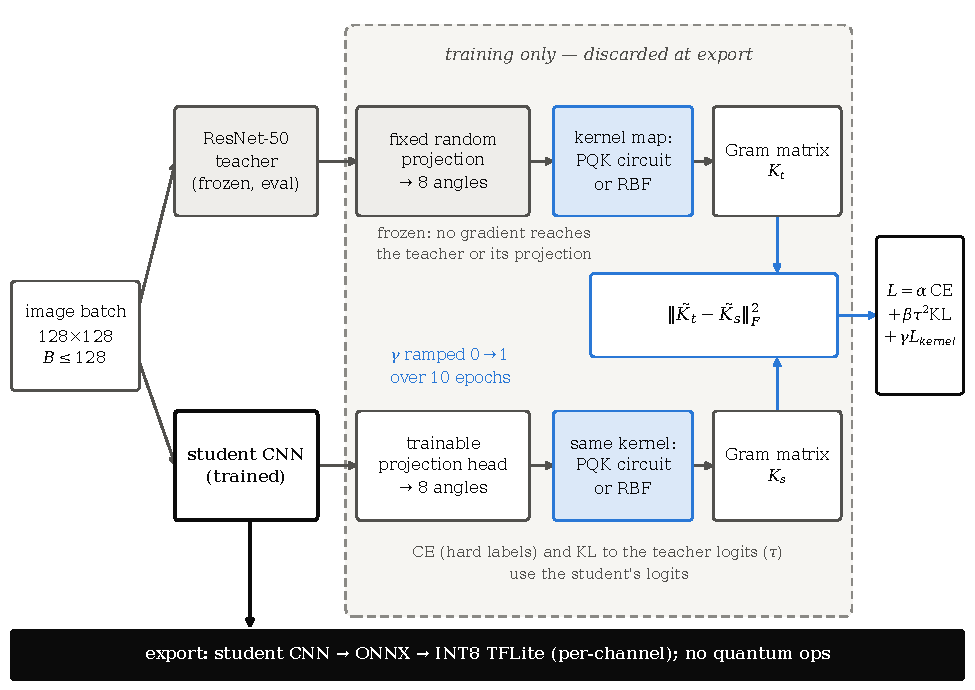
\includegraphics[width=\textwidth]{pipeline}
  \caption{Training-time pipeline. Penultimate features of the frozen teacher and of the student are projected to eight angles and compared through the Gram matrices of one kernel (the PQK circuit or an RBF kernel). Everything inside the dashed region is discarded at export; only the student CNN is deployed.}
  \label{fig:pipeline}
\end{figure*}

Let $x$ be an image with label $y$, let $z_t(x)\in\mathbb{R}^{2048}$ and $z_s(x)\in\mathbb{R}^{d_s}$ be the penultimate features of the teacher and the student, and let $\ell_t,\ell_s$ be their logits.
All losses are computed on batches of up to $B=128$ images; the last batch of an epoch is smaller, and the $33$-image RPS-25 validation split is a single batch.

\subsection{Baseline objectives}
\label{sec:objectives}

\Scratch minimizes the cross-entropy $\mathrm{CE}(\ell_s,y)$.
\Kd is Hinton distillation~\citep{hinton2015distilling},
\begin{equation}
  \begin{split}
  L_{\mathrm{KD}} ={}& \alpha\,\mathrm{CE}(\ell_s,y)\\
  &+ \beta\,\tau^{2}\,\mathrm{KL}\!\left(\mathrm{softmax}(\ell_t/\tau)\,\Vert\,\mathrm{softmax}(\ell_s/\tau)\right),
  \end{split}
\end{equation}
with $\alpha=\beta=0.5$ and a temperature $\tau$ that was screened on some pairs and reused on others (Table~\ref{tab:hparams-methods}).
\Rkd~\citep{park2019relational} adds distance-wise and angle-wise relational terms on the penultimate features,
\begin{equation}
  \begin{split}
  L_{\mathrm{RKD}} ={}& \mathrm{CE}(\ell_s,y) + w_d\,\mathrm{SmoothL1}\big(\psi_D(z_s),\psi_D(z_t)\big)\\
  &+ w_a\,\mathrm{SmoothL1}\big(\psi_A(z_s),\psi_A(z_t)\big),
  \end{split}
\end{equation}
where $\psi_D$ collects the pairwise distances of a batch normalized by their mean and $\psi_A$ the cosines of the angles formed by triplets.
Both potentials are dimension-free, so a 2048-dimensional teacher and a student of any width can be compared directly.

\subsection{Kernel alignment}
\label{sec:kernel-alignment}

The two kernel methods (\Pqk and its twin \Rbf) add a kernel-alignment term to the logit objective,
\begin{equation}
  L = \alpha\,\mathrm{CE}(\ell_s,y) + \beta\,\tau^{2}\,\mathrm{KL}(\cdot) + \gamma_e\,L_{\mathrm{kernel}},
  \label{eq:loss}
\end{equation}
\begin{equation}
  L_{\mathrm{kernel}} = \big\Vert \tilde K_t - \tilde K_s \big\Vert_F^{2},\qquad
  \tilde K = \frac{K}{\operatorname{tr}K},
\end{equation}
with $\alpha=\beta=0.5$, a single temperature $\tau=0.5$ for all kernel methods, and the weight $\gamma_e=\gamma_{\max}\min\!\big(1,(e{+}1)/10\big)$ ramped linearly over the first ten epochs $e$, with $\gamma_{\max}=1$.
Validation is always scored at $\gamma_{\max}$ so that the ramp cannot change which checkpoint is selected.
$K_t$ and $K_s$ are the $B\times B$ Gram matrices of the teacher and the student, built from eight angles per image,
\begin{equation}
  \theta_s = \pi\,\sigma(W_s z_s + b_s),\quad
  \theta_t = \pi\,\sigma(W_t z_t + b_t),\quad \theta\in[0,\pi]^{8}.
\end{equation}
The student-side projection $(W_s,b_s)$ is trained jointly with the student, and gradients reach the student through the kernel.
The teacher-side projection $(W_t,b_t)$ is drawn at default initialization at the start of each run, frozen, and evaluated without gradients.
Freezing it is necessary. If both projections are trainable, collapsing both to constant maps sets every Gram entry to one and makes the two normalized matrices identical. The loss $L_{\mathrm{kernel}}$ then reaches exactly zero without the student learning anything.
Our first implementation had this flaw. In the first \Pqk run we inspected (RPS-25, LeNet-5, seed~0) the mean off-diagonal kernel value was \CollapseStudent{} for the student and \CollapseTeacher{} for the teacher\extra{; Appendix~\ref{app:pitfalls} gives the details}.
We log the mean off-diagonal kernel value in every epoch and treat values below $0.05$ or above $0.95$ as degenerate.

\subsection{The projected quantum kernel}
\label{sec:pqk}

\begin{figure*}[t]
  \centering
  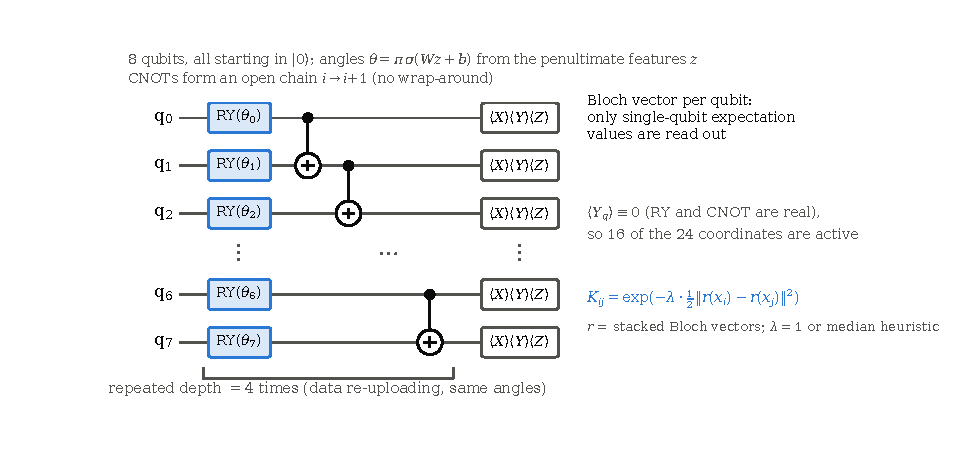
\includegraphics[width=\textwidth]{pqk_circuit}
  \caption{The fixed feature map behind \Pqk (shown for qubits $0$, $1$, $2$ and $7$). Each of the eight angles drives an $R_Y$ rotation, followed by an open chain of CNOT gates; the pair is repeated $4$ times with the same angles. Only single-qubit expectation values are read out. Nothing in the circuit is trainable.}
  \label{fig:circuit}
\end{figure*}

The quantum kernel is the projected quantum kernel of Huang et al.~\citep{huang2021power}.
The circuit (Figure~\ref{fig:circuit}) applies $R_Y(\theta_q)$ to every qubit $q$ and then a CNOT from qubit $q$ to $q{+}1$ for $q=0,\dots,6$, and repeats this pair of layers $4$ times on $8$ qubits starting from $|0\rangle^{\otimes 8}$.
The CNOTs form an open chain, with no gate closing it into a ring.
For each input the Bloch vector of every qubit is measured, $r(\theta)=(\langle X_q\rangle,\langle Y_q\rangle,\langle Z_q\rangle)_{q=0}^{7}$.
Because $R_Y$ and CNOT are real matrices, the state stays real and $\langle Y_q\rangle\equiv0$, so only $16$ of the $24$ coordinates are active.
The kernel compares inputs through their single-qubit reduced states $\rho_q=\tfrac12(I+r_q\cdot\sigma)$,
\begin{equation}
  \begin{split}
  K(\theta,\theta') &= \exp\!\Big(-\lambda\sum_{q}\big\Vert\rho_q(\theta)-\rho_q(\theta')\big\Vert_F^{2}\Big)\\
  &= \exp\!\Big(-\tfrac{\lambda}{2}\,\big\Vert r(\theta)-r(\theta')\big\Vert^{2}\Big),
  \end{split}
  \label{eq:pqk}
\end{equation}
where the second form follows from $\operatorname{tr}(\sigma_a\sigma_b)=2\delta_{ab}$.
The readout is restricted to single-qubit expectation values. At eight qubits the circuit is cheap to simulate exactly, so the kernel is classically tractable at this size. We use PennyLane~\citep{bergholm2018pennylane} on its state-vector \texttt{lightning.qubit} backend with adjoint differentiation.

The scale $\lambda$ is handled in two ways.
\Pqk uses the pre-specified $\lambda=1$.
The variant \texttt{pqk\_adaptive}, adopted after the first results (Section~\ref{sec:setup-protocol}), sets $\lambda$ in every batch so that $K=\exp\!\big(-d^{2}/(2m)\big)$ with $d^{2}=\tfrac12\Vert\Delta r\Vert^{2}$ and $m$ the median off-diagonal $d^{2}$ of the batch.
With this choice the Gram matrix is the median-heuristic RBF kernel on the measured features $r(\theta)$.

\subsection{Matched classical controls}
\label{sec:controls}

\Rbf is the same pipeline with an RBF kernel, $K=\exp\!\big(-\Vert\theta-\theta'\Vert^{2}/(2m)\big)$, on the same eight angles with the same median heuristic.
The quantum branch with adaptive $\lambda$ and \Rbf therefore differ only in the map $\theta\mapsto r(\theta)$ that precedes an identically calibrated RBF kernel.
Two further arms isolate where an effect of that map could come from.
\begin{itemize}
  \item \texttt{noent\_control} deletes the CNOT gates from the circuit.
  Each qubit then sees $R_Y(\theta_q)^{4}=R_Y(4\theta_q)$, so $r=(\sin4\theta_q,0,\cos4\theta_q)$ exactly (checked against the simulator to $6\times10^{-8}$), with the same $16$ active coordinates and range, no trainable parameters and the same adaptive RBF kernel. It differs from \texttt{pqk\_adaptive} only by entanglement.
  \item \texttt{pqk\_fit} and \texttt{rbf\_fit} replace the random teacher-side projection by a map fitted once on the training split and then frozen: the $C{-}1$ shrinkage-LDA directions, completed to eight outputs with the leading principal components of the residual and standardized on the training set.
\end{itemize}
A third control, random Fourier features drawn from the circuit's own frequency spectrum, was implemented but not run\extra{ (Section~\ref{sec:limitations})}.
Table~\ref{tab:kernel-cfg} lists the settings of every kernel arm.

\begin{table*}[t]
  \centering
  \caption{Kernel arms. All use eight angles, the loss of Eq.~\eqref{eq:loss} and the same frozen teacher.}
  \label{tab:kernel-cfg}
  \adjustbox{max width=\textwidth}{\begin{tabular}{@{}llrrll@{}}
\toprule
Method & Kernel on the 8 angles & Qubits & Depth & $\lambda$ / bandwidth & Teacher projection \\
\midrule
\texttt{rbf\_control} & RBF & 8 & -- & median heuristic & random (frozen) \\
\texttt{pqk} & projected quantum (RY+CNOT) & 8 & 4 & 1 & random (frozen) \\
\texttt{pqk\_adaptive} & projected quantum (RY+CNOT) & 8 & 4 & median heuristic & random (frozen) \\
\texttt{noent\_control} & classical map $[\sin4\theta,\cos4\theta]$ & 8 & 4 & median heuristic & random (frozen) \\
\texttt{pqk\_fit} & projected quantum (RY+CNOT) & 8 & 4 & median heuristic & LDA+PCA (fitted, frozen) \\
\texttt{rbf\_fit} & RBF & 8 & -- & median heuristic & LDA+PCA (fitted, frozen) \\
\bottomrule
\end{tabular}
}
\end{table*}

\subsection{What is trained and what is deployed}
\label{sec:deployed}

Only the student CNN is exported.
The projection heads, the circuit and the kernels exist only inside the training loop, and a purity check on the exported graph fails if any of them is present (Section~\ref{sec:setup-int8}).
The deployed model of every method, including \Pqk, is therefore an ordinary convolutional network, and the quantum kernel affects it only through the weights it learned.

\section{Experimental Setup}
\label{sec:setup}

\subsection{Data}
\label{sec:setup-data}

\begin{figure*}[t]
  \centering
  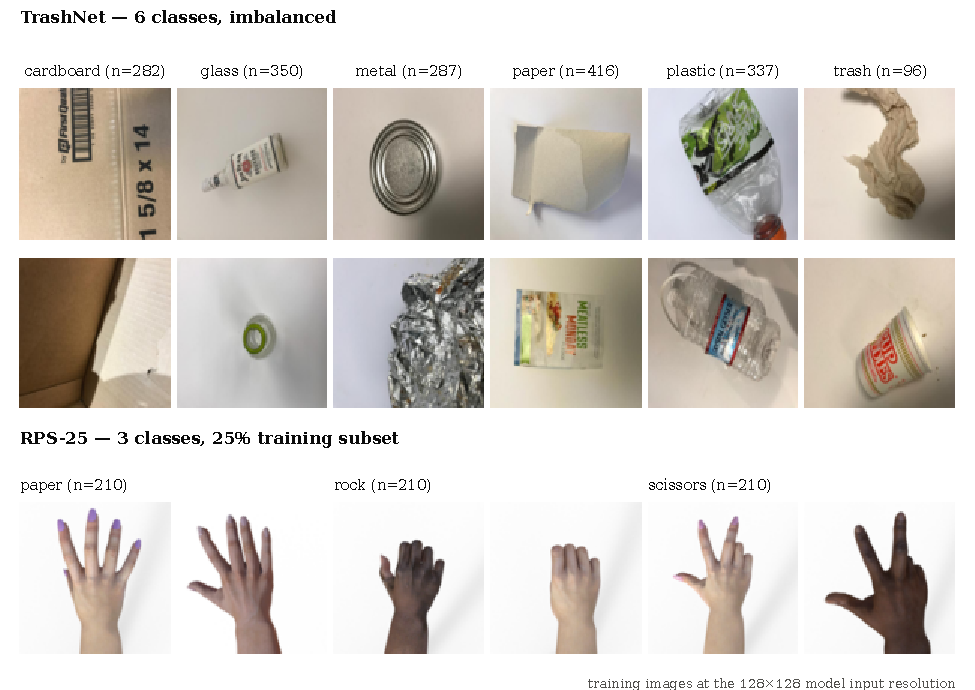
\includegraphics[width=\textwidth]{dataset_samples}
  \caption{Training images from the two datasets at the $128{\times}128$ input resolution, two per class, and the number of training images per class.}
  \label{fig:samples}
\end{figure*}

\begin{table*}[t]
  \centering
  \caption{Datasets and splits.}
  \label{tab:data}
  \adjustbox{max width=\textwidth}{\begin{tabular}{@{}lrrrrrll@{}}
\toprule
Dataset & Classes & Train & Val & Test & Smallest / largest train class & Train sampler & Primary metric \\
\midrule
TrashNet & 6 & 1{,}768 & 379 & 380 & trash 96 / paper 416 & class-balanced (weighted) & macro-F1 \\
RPS-25 & 3 & 630 & 33 & 372 & 210 / 210 (balanced) & shuffle & top-1 accuracy \\
\bottomrule
\end{tabular}
}
\end{table*}

\textbf{TrashNet}~\citep{yang2016trashnet} has \(2{,}527\) photographs in six classes (cardboard, glass, metal, paper, plastic, trash) and no official split.
We split it once, stratified $70/15/15$ with seed $0$, cache the split, and never re-split.
The classes are imbalanced (Table~\ref{tab:data}). Macro-F1 is therefore the primary metric, with accuracy as secondary, and training batches are drawn with a class-balanced sampler instead of class-weighted cross-entropy.
\textbf{RPS-25} is a $25\%$ subset of the training images of the Rock--Paper--Scissors dataset~\citep{moroney2019rps}. We chose it to be deliberately low-data so that distillation has room to help.
It keeps the official validation (33 images) and test (372 images) splits, and top-1 accuracy is its primary metric.
The two datasets differ in nature as well as size. RPS-25 is a three-class gesture task with clean backgrounds, and TrashNet is a six-class material task with imbalance. We treat RPS-25 as a low-data confirmation, not as a second application.
All images are resized to $128{\times}128$ and normalized with ImageNet statistics.
Training images use random resized crops, RandAugment~\citep{cubuk2020randaugment} and horizontal flips, with the strengths in Table~\ref{tab:hparams-students}. These are identical for every method.

\subsection{Teacher and students}
\label{sec:setup-models}

The teacher is an ImageNet-pretrained ResNet-50~\citep{he2016deep}, fine-tuned once per dataset and then frozen in evaluation mode with gradients disabled. Fine-tuning uses AdamW~\citep{loshchilov2019decoupled} with learning rate $10^{-4}$, weight decay $10^{-4}$, a cosine schedule, batch $128$, at most $20$ epochs and patience $5$, and selects by validation macro-F1.
Its test macro-F1 is \TeacherTn{} on TrashNet and \TeacherRps{} on RPS-25.
The students are trained from random initialization. They are MobileNetV2 with width multiplier $0.35$ (0.40\,M parameters), MobileNetV3-Small (0.93\,M) and a LeNet-5~\citep{lecun1998gradient} variant with global average pooling before the classifier (0.03\,M).
MobileNetV2-0.35 and MobileNetV3-Small are the edge-relevant students and the only ones exported. LeNet-5 serves as a capacity floor.

\subsection{Training protocol}
\label{sec:setup-training}

\begin{table*}[t]
  \centering
  \caption{Student recipes. BN: batch-normalization statistics are either the usual running estimates or the per-batch statistics used during training with a recalibration pass on clean training images before every evaluation (needed when an epoch has too few batches, or for MobileNetV3-Small's Hardswish and squeeze-excite blocks, to keep running statistics stable). RRC: minimum scale of the random resized crop. $^{*}$One of the three seeds used a different budget\extra{ (Appendix~\ref{app:recipe})}.}
  \label{tab:hparams-students}
  \adjustbox{max width=\textwidth}{\begin{tabular}{@{}llrrrcccc@{}}
\toprule
Dataset & Student & Epochs & Patience & LR & BN stats & RRC min scale & RandAugment (ops, mag.) \\
\midrule
TrashNet & MobileNetV2-0.35 & 60 & 10 & $0.001$ & running & 0.85 & 1, 5 \\
TrashNet & MobileNetV3-S & 40 & 8 & $0.001$ & per-batch + recal. & 0.85 & 1, 5 \\
TrashNet & LeNet-5 & 60 & 12 & $0.001$ & running & 0.85 & 1, 5 \\
RPS-25 & MobileNetV2-0.35 & 60 & 10 & $0.001$ & per-batch + recal. & 0.7 & 2, 9 \\
RPS-25 & MobileNetV3-S & 40 & 8 & $0.001$ & per-batch + recal. & 0.7 & 2, 9 \\
RPS-25 & LeNet-5 & 40/60$^{*}$ & 8/12 & $0.001$ & per-batch + recal. & 0.7 & 2, 9 \\
\bottomrule
\end{tabular}
}
\end{table*}

All methods on a pair share the data, the optimizer (AdamW, weight decay $10^{-4}$, cosine learning-rate schedule), the batch size ($128$), the epoch budget and the early-stopping patience (Table~\ref{tab:hparams-students}). The best validation checkpoint is restored.
Two cells depart from this\extra{ and are disclosed in Appendix~\ref{app:recipe}}. One \Scratch seed on RPS-25/LeNet-5 used a different budget, and the \Kd cell for that pair mixes two temperatures.
Checkpoints are selected by validation macro-F1 on TrashNet. On RPS-25 they are selected by validation loss, because the $33$-image validation split makes validation F1 too erratic to select on.
That validation loss is each method's own training objective evaluated on the validation batch. For the kernel methods it includes the kernel term at $\gamma_{\max}$, computed on a single $33$-image Gram matrix.
Each cell is trained with seeds $0$, $1$ and $2$, which set the student initialization, the data order and the random teacher projection.
Table~\ref{tab:hparams-methods} lists the loss settings that were used.

\begin{table*}[t]
  \centering
  \caption{Loss settings recorded in the runs. Kernel methods share $\tau=0.5$, whereas the \Kd temperature was screened on some pairs and reused on others (see text). $^{\P}$The seeds of this cell used different settings\extra{ (Appendix~\ref{app:recipe})}.}
  \label{tab:hparams-methods}
  \adjustbox{max width=\textwidth}{\begin{tabular}{@{}lll@{}}
\toprule
Method & Loss setting & Pairs \\
\midrule
\texttt{scratch} & CE$\times$1 & all pairs \\
\texttt{kd} & $\alpha{=}0.5$, $\beta{=}0.5$, $\tau{=}3$ & TrashNet (all students) \\
 & $\alpha{=}0.5$, $\beta{=}0.5$, $\tau{=}1$ & RPS-25: MobileNetV2-0.35, MobileNetV3-S \\
 & $\alpha{=}0.5$, $\beta{=}0.5$, $\tau{=}0.5$ & RPS-25: LeNet-5 (seed 0)$^{\P}$ \\
 & $\alpha{=}0.5$, $\beta{=}0.5$, $\tau{=}1$ & RPS-25: LeNet-5 (seeds 1, 2)$^{\P}$ \\
\texttt{rkd} & CE$\times$1, dist.$\times$5, angle$\times$10 & TrashNet: MobileNetV2-0.35, MobileNetV3-S; RPS-25: MobileNetV2-0.35, MobileNetV3-S \\
 & CE$\times$1, dist.$\times$1, angle$\times$2 & TrashNet: LeNet-5 \\
\texttt{rbf\_control} & $\alpha{=}0.5$, $\beta{=}0.5$, $\tau{=}0.5$, $\gamma{=}1$ (10-epoch ramp) & all pairs \\
\texttt{pqk} & $\alpha{=}0.5$, $\beta{=}0.5$, $\tau{=}0.5$, $\gamma{=}1$ (10-epoch ramp) & all pairs \\
\texttt{pqk\_adaptive} & $\alpha{=}0.5$, $\beta{=}0.5$, $\tau{=}0.5$, $\gamma{=}1$ (10-epoch ramp) & all pairs \\
\texttt{noent\_control} & $\alpha{=}0.5$, $\beta{=}0.5$, $\tau{=}0.5$, $\gamma{=}1$ (10-epoch ramp) & TrashNet: MobileNetV2-0.35, MobileNetV3-S; RPS-25: MobileNetV2-0.35, MobileNetV3-S \\
\bottomrule
\end{tabular}
}
\end{table*}

\subsection{Selection, reporting and the status of the results}
\label{sec:setup-protocol}

Every number is the mean $\pm$ sample standard deviation ($n{-}1$) over three seeds.
Comparisons are paired by seed. We report the mean paired difference, its standard deviation and the number of seeds on which the first method is ahead.
Two-sided paired $t$-tests are given as descriptive summaries and are not corrected for multiple comparisons.
For the follow-up arms (\texttt{pqk\_adaptive}, \texttt{noent\_control}, \texttt{pqk\_fit}, \texttt{rbf\_fit}) we checked that a shared seed means identical student initialization and data order, because the first-batch cross-entropy and KL gradients are identical across the arms. The stored gradient logs confirm this for \texttt{noent\_control}, \texttt{pqk\_fit} and \texttt{rbf\_fit} in every cell. For \texttt{pqk\_adaptive} the check was made when the arms were set up, and its logs were stored for two runs only.
For the earlier grid, pairing means a shared seed value only.

These results are exploratory, for three reasons.
First, several design choices were screened on seed~0, and some were judged by test-split scores. These are the student recipes (sampler, augmentation strength and epoch budget, tuned on MobileNetV2 for TrashNet), the KD temperature, and the RKD weights.
Second, the temperature of the kernel methods ($\tau=0.5$) was inherited from a KD screen on LeNet-5 with RPS-25 and was not re-tuned per pair. The \Kd temperature was screened on TrashNet/MobileNetV2-0.35 ($\tau=3$) and RPS-25/MobileNetV2-0.35 ($\tau=1$) and reused for the other students of the dataset (RPS-25/LeNet-5 is a special case\extra{, Appendix~\ref{app:recipe}}). Comparisons between a kernel method and \Kd are therefore not matched on that parameter, and may disadvantage the kernel methods.
Third, the choice of $\lambda$ for \Pqk was made after results were seen. The pre-specified $\lambda=1$ gave the \Pqk results of the first full grid. The adaptive $\lambda$ was adopted afterwards, per pair, by the higher three-seed \emph{validation} macro-F1 of the two variants\extra{ (Appendix~\ref{app:screens})}.
For the choice of $\lambda$ and for the follow-up analyses, validation scores decide and test scores are descriptive. The headline comparisons show both $\lambda$ variants.
A confirmatory claim would need a frozen protocol, selection on validation alone and fresh data, which we do not have.

\subsection{INT8 export}
\label{sec:setup-int8}

Each trained MobileNet student is exported in three steps. The projection and kernel modules are stripped, the PyTorch graph is converted to ONNX (opset 17, static batch size 1), and ONNX is converted to a fully integer TFLite model with per-channel weight quantization. Calibration uses $256$ unaugmented training images, and input and output are quantized to INT8.
Four checks run on every model: a purity check that the graph contains no projection, quantum or custom operations; a check that every convolution is quantized per channel and the whole graph is integer; ONNX--PyTorch parity on the logits; and reload of the fp32 weights reproducing the recorded test score.
The INT8 test score is measured with the LiteRT interpreter on an x86 PC, whose default and builtin kernels give identical outputs (``PC'' below).
The exported set contains $\NIntModels{}$ models: two students, two datasets, five methods and three seeds, plus the second $\lambda$ variant of \Pqk on the two pairs where both were exported.
For \Pqk the exported variant is the one the validation rule had chosen at export time. For TrashNet with MobileNetV2 that was $\lambda=1$, whereas the final rule prefers adaptive $\lambda$, which has no INT8 export (marked $\ddagger$ in the tables).

\subsection{On-device benchmark}
\label{sec:setup-device}

The INT8 models run on a Raspberry Pi~4 Model~B (Cortex-A72, four cores, 4\,GB, Ubuntu 20.04, \texttt{ondemand} governor, 600--1800\,MHz) with LiteRT (\texttt{ai-edge-litert} 2.1.0, Python 3.13).
Each model runs in a fresh process with $50$ warm-up and $500$ timed invocations at batch size~1, and every run starts below $55\,^\circ$C.
We log invocation latency percentiles, the full quantize--invoke--dequantize pipeline, load and cold-start time, CPU use, resident memory, and SoC temperature and clock every $100$\,ms. We also read the firmware's throttling flags before and after each timed window.
The suite covers all models with the default XNNPACK delegate and with the builtin kernels only, a thread sweep from one to four threads, and fp32 references.
Each model is also scored on the full test split on the device and compared with the PC's logits.
A live USB-camera pipeline ($640{\times}480$, MJPEG) measures the end-to-end cost including image preparation.
Energy was not measured because no power meter was attached, and the Jetson Orin Nano and ESP32-S3 targets were not benchmarked.

\subsection{Compute}
\label{sec:setup-compute}

All training ran on a single GPU, with several runs often sharing it. Per-epoch wall-clock times are therefore not comparable across methods, and we report compute-hours instead (Section~\ref{sec:results-cost}).
The $152$ student runs in the results include, besides the grid, the follow-up arms, the screens\extra{ of Appendix~\ref{app:screens}} and seven runs of two wider MobileNetV2 variants (width multipliers $0.5$ and $0.6$). Those seven were stopped as incomplete capacity probes and are not reported.

\section{Results}
\label{sec:results}

\subsection{Distillation baselines}
\label{sec:results-baselines}

\begin{table*}[t]
  \centering
  \caption{Test macro-F1 and top-1 accuracy, mean $\pm$ sample std over three seeds. Bold: best mean in a column within a student. $^{\dagger}$\Pqk with the validation-selected adaptive $\lambda$ (elsewhere $\lambda=1$). $^{\S}$One of the three seeds used a different training budget, and $^{\P}$the seeds of the \Kd cell used two different temperatures\extra{ (Appendix~\ref{app:recipe})}. \Rkd was not part of the final grid for RPS-25/LeNet-5. The primary metric is macro-F1 on TrashNet and top-1 on RPS-25.}
  \label{tab:main}
  \adjustbox{max width=\textwidth}{\begin{tabular}{@{}llcccc@{}}
\toprule
 & & \multicolumn{2}{c}{TrashNet (6 classes)} & \multicolumn{2}{c}{RPS-25 (3 classes)} \\
\cmidrule(lr){3-4}\cmidrule(lr){5-6}
Student & Method & Macro-F1 & Top-1 & Macro-F1 & Top-1 \\
\midrule
MobileNetV2-0.35 & \texttt{scratch} & $0.684\pm0.014$ & $0.697\pm0.021$ & $0.710\pm0.023$ & $0.727\pm0.030$ \\
 & \texttt{kd} & $\mathbf{0.708}\pm0.013$ & $\mathbf{0.725}\pm0.009$ & $0.710\pm0.088$ & $0.719\pm0.087$ \\
 & \texttt{rkd} & $0.672\pm0.004$ & $0.686\pm0.003$ & $\mathbf{0.737}\pm0.051$ & $\mathbf{0.745}\pm0.048$ \\
 & \texttt{rbf\_control} & $0.671\pm0.010$ & $0.692\pm0.012$ & $0.684\pm0.062$ & $0.702\pm0.059$ \\
 & \texttt{pqk} & $0.683\pm0.013$$^{\dagger}$ & $0.694\pm0.016$$^{\dagger}$ & $0.713\pm0.030$$^{\dagger}$ & $0.730\pm0.019$$^{\dagger}$ \\
\midrule
MobileNetV3-S & \texttt{scratch} & $0.724\pm0.016$ & $0.745\pm0.016$ & $0.816\pm0.053$ & $0.828\pm0.045$ \\
 & \texttt{kd} & $\mathbf{0.732}\pm0.020$ & $\mathbf{0.753}\pm0.021$ & $0.830\pm0.089$ & $0.843\pm0.075$ \\
 & \texttt{rkd} & $0.716\pm0.003$ & $0.736\pm0.007$ & $0.849\pm0.048$ & $0.859\pm0.041$ \\
 & \texttt{rbf\_control} & $0.715\pm0.037$ & $0.730\pm0.040$ & $\mathbf{0.888}\pm0.063$ & $\mathbf{0.892}\pm0.060$ \\
 & \texttt{pqk} & $0.718\pm0.009$$^{\dagger}$ & $0.735\pm0.008$$^{\dagger}$ & $0.840\pm0.065$ & $0.851\pm0.054$ \\
\midrule
LeNet-5 & \texttt{scratch} & $0.529\pm0.021$ & $0.541\pm0.022$ & $\mathbf{0.676}\pm0.108$$^{\S}$ & $\mathbf{0.676}\pm0.109$$^{\S}$ \\
 & \texttt{kd} & $0.484\pm0.074$ & $0.490\pm0.075$ & $0.650\pm0.012$$^{\P}$ & $0.652\pm0.016$$^{\P}$ \\
 & \texttt{rkd} & $\mathbf{0.578}\pm0.016$ & $\mathbf{0.597}\pm0.021$ & -- & -- \\
 & \texttt{rbf\_control} & $0.539\pm0.008$ & $0.552\pm0.007$ & $0.538\pm0.202$ & $0.584\pm0.153$ \\
 & \texttt{pqk} & $0.535\pm0.003$ & $0.552\pm0.003$ & $0.638\pm0.070$ & $0.642\pm0.058$ \\
\bottomrule
\end{tabular}
}
\end{table*}

\begin{figure*}[t]
  \centering
  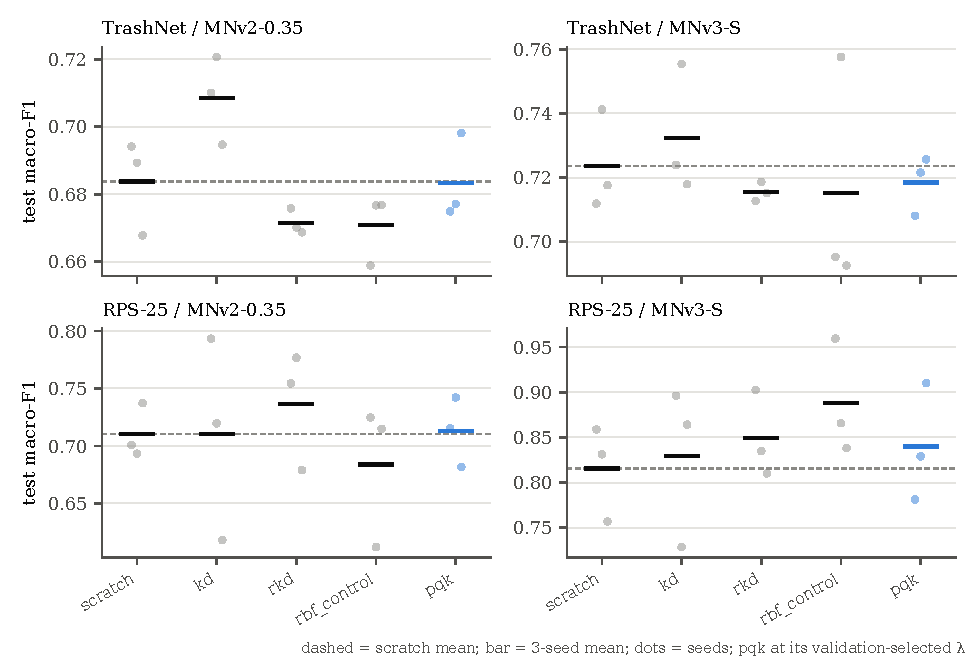
\includegraphics[width=0.95\textwidth]{methods_seeds}
  \caption{Test macro-F1 of the five methods for the four MobileNet pairs. Dots are individual seeds, bars are means, and the dashed line is the mean of \Scratch.}
  \label{fig:methods}
\end{figure*}

Table~\ref{tab:main} and Figure~\ref{fig:methods} give the baseline picture.
Distillation helps in some pairs and not in others.
\Kd beats \Scratch on TrashNet for both MobileNets, by $+0.025\pm0.008$ (MobileNetV2-0.35) and $+0.009\pm0.007$ (MobileNetV3-Small) macro-F1, ahead on all three seeds of each. On the $0.03$\,M LeNet-5 it hurts ($-0.045\pm0.093$), and \Rkd helps ($+0.049\pm0.035$, three of three seeds).
\Rkd is slightly behind \Scratch on the TrashNet MobileNets ($-0.012$ and $-0.008$).
No method dominates.
The best mean is \Kd on the TrashNet MobileNets, \Rkd on TrashNet/LeNet-5 and RPS-25/MobileNetV2-0.35, \Rbf on RPS-25/MobileNetV3-Small, and \Scratch on RPS-25/LeNet-5. \Pqk is the best method on no pair.
The classical kernel-alignment arm \Rbf beats \Scratch on the mean in only \RbfBeatsScratch{} of \NPairs{} pairs. On RPS-25/MobileNetV3-Small it does so clearly ($+0.072\pm0.034$, three of three seeds).
On TrashNet all students stay well below the teacher: the best reaches $0.732$ macro-F1 against $0.876$. On RPS-25 the best student (the RBF twin with MobileNetV3-Small, $0.888$) comes close to the teacher's $0.907$.
Seed noise is large relative to these effects, particularly on RPS-25, where the standard deviation across seeds ranges from $0.012$ to $0.202$, against $0.003$ to $0.074$ on TrashNet.

\subsection{PQK against logit KD, the RBF twin and relational KD}
\label{sec:results-pqk}

\begin{table*}[t]
  \centering
  \caption{Paired difference $\mathtt{pqk}-\mathtt{kd}$ in test macro-F1 (mean $\pm$ std of the per-seed differences, and the number of seeds on which \Pqk is ahead). \Pqk is at its validation-selected $\lambda$ at fp32 and at the exported variant at INT8; these differ only for TrashNet/MobileNetV2-0.35, where the INT8 models use $\lambda=1$ and the fp32 column adaptive $\lambda$. $^{\P}$The \Kd cell for RPS-25/LeNet-5 mixes two temperatures\extra{ (Appendix~\ref{app:recipe})}. ``PC'' uses LiteRT's builtin kernels on x86; ``Pi'' columns were measured on the Raspberry Pi, with its builtin kernels and with its default XNNPACK delegate. LeNet-5 was not exported.}
  \label{tab:pqk-kd}
  \adjustbox{max width=\textwidth}{\begin{tabular}{@{}llcccc@{}}
\toprule
 & & fp32 & \multicolumn{3}{c}{INT8} \\
\cmidrule(lr){4-6}
Dataset & Student & test macro-F1 & PC (builtin) & Pi builtin & Pi XNNPACK \\
\midrule
TrashNet & MobileNetV2-0.35 & $-0.025\pm0.025$ (1/3) & $+0.004\pm0.006$ (2/3) & $+0.004\pm0.006$ (2/3) & $-0.004\pm0.010$ (1/3) \\
TrashNet & MobileNetV3-S & $-0.014\pm0.021$ (1/3) & $-0.017\pm0.021$ (0/3) & $-0.016\pm0.016$ (0/3) & $-0.025\pm0.015$ (0/3) \\
TrashNet & LeNet-5 & $+0.051\pm0.073$ (2/3) & -- & -- & -- \\
RPS-25 & MobileNetV2-0.35 & $+0.003\pm0.073$ (2/3) & $+0.025\pm0.108$ (2/3) & $+0.025\pm0.108$ (2/3) & $+0.032\pm0.113$ (2/3) \\
RPS-25 & MobileNetV3-S & $+0.010\pm0.112$ (2/3) & $+0.016\pm0.101$ (2/3) & $+0.017\pm0.104$ (2/3) & $+0.011\pm0.115$ (2/3) \\
RPS-25 & LeNet-5 & $-0.013\pm0.059$ (2/3)$^{\P}$ & -- & -- & -- \\
\midrule
\multicolumn{2}{@{}l}{Pairs where \texttt{pqk} is ahead on the mean} & 3/6 & 3/4 & 3/4 & 2/4 \\
\bottomrule
\end{tabular}
}
\end{table*}

\begin{figure*}[t]
  \centering
  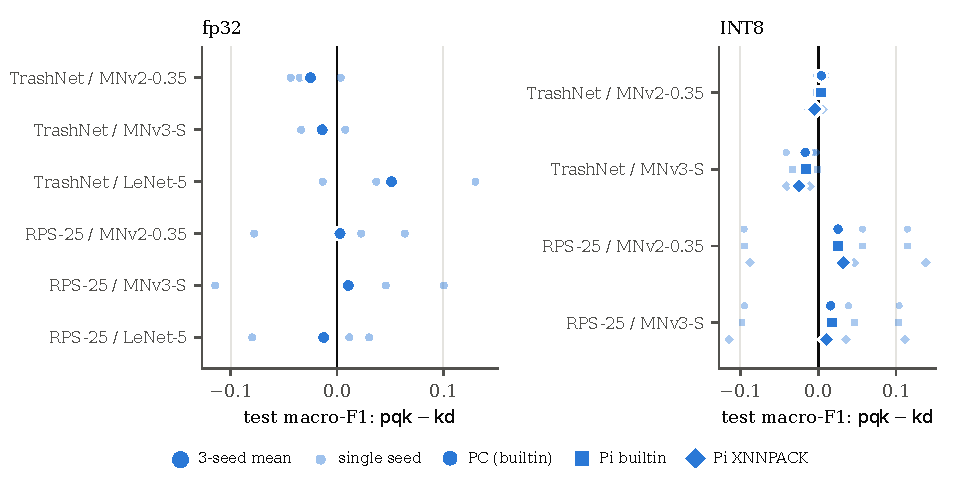
\includegraphics[width=\textwidth]{pqk_vs_kd}
  \caption{$\mathtt{pqk}-\mathtt{kd}$ per pair, paired by seed, at fp32 (left) and after INT8 conversion under three sets of kernels (right). Positive values favour \Pqk.}
  \label{fig:pqk-kd}
\end{figure*}

\paragraph{Against logit KD.}
Table~\ref{tab:pqk-kd} and Figure~\ref{fig:pqk-kd} show that \Pqk and \Kd cannot be told apart.
At fp32, \Pqk is ahead of \Kd on the mean in \KdAheadFp{} of \NPairs{} pairs. The count is \KdAheadFpEx{} if the one \Kd seed trained at a different temperature on RPS-25/LeNet-5 is excluded\extra{ (Appendix~\ref{app:recipe})}.
On TrashNet, the primary dataset, \Pqk is behind on both MobileNets, by $0.025\pm0.025$ and $0.014\pm0.021$ macro-F1, and ahead on one seed of three in each.
It is ahead on TrashNet/LeNet-5 ($+0.051\pm0.073$), where \Kd itself fails. On RPS-25 it is ahead by $+0.003\pm0.073$ (MobileNetV2-0.35) and $+0.010\pm0.112$ (MobileNetV3-Small) and behind on LeNet-5 ($-0.013\pm0.059$). On top-1, the primary metric there, the three differences are $+0.012$, $+0.008$ and $-0.010$.
After INT8 conversion, \Pqk is ahead of \Kd on the mean in \KdAheadPc{} of \NExported{} pairs on PC numerics and on the Pi's builtin kernels, and in \KdAheadXnn{} of \NExported{} on the Pi's default XNNPACK kernels.
TrashNet/MobileNetV3-Small is a loss under all three sets of kernels ($-0.017$, $-0.016$, $-0.025$, with \Pqk behind on every seed). The RPS-25 differences ($+0.011$ to $+0.032$) come with paired standard deviations of $0.10$ to $0.12$.
No difference is significant. The smallest uncorrected paired $p$-value is \MinPKd{} at fp32 and \MinPKdInt{} at INT8.
One caveat applies: the \Kd temperature was screened on some pairs, whereas the kernel methods use one untuned $\tau$ (Section~\ref{sec:setup-protocol}). This comparison is therefore not matched on that parameter.
Against \Scratch, \Pqk differs by between $-0.039$ and $+0.024$ across the six pairs, with a smallest $p$-value of \MinPScratch{}.

\begin{table*}[t]
  \centering
  \caption{Test macro-F1 of the twin \Rbf and the paired difference $\mathtt{pqk}-\mathtt{rbf\_control}$ for the two $\lambda$ calibrations of \Pqk. Adaptive $\lambda$ has only one seed on the two LeNet-5 pairs and is omitted there. $^{\S}$See Table~\ref{tab:main}.}
  \label{tab:g2}
  \adjustbox{max width=\textwidth}{\begin{tabular}{@{}llccccc@{}}
\toprule
Dataset & Student & \texttt{scratch} & \texttt{rbf\_control} & $\Delta$ \texttt{pqk} ($\lambda{=}1$) & $\Delta$ \texttt{pqk} (adaptive $\lambda$) & selected \\
\midrule
TrashNet & MobileNetV2-0.35 & $0.684\pm0.014$ & $0.671\pm0.010$ & $+0.023\pm0.016$ (3/3) & $+0.013\pm0.011$ (3/3) & adaptive \\
TrashNet & MobileNetV3-S & $0.724\pm0.016$ & $0.715\pm0.037$ & $-0.042\pm0.049$ (1/3) & $+0.003\pm0.036$ (2/3) & adaptive \\
TrashNet & LeNet-5 & $0.529\pm0.021$ & $0.539\pm0.008$ & $-0.004\pm0.010$ (2/3) & -- & $\lambda{=}1$ \\
RPS-25 & MobileNetV2-0.35 & $0.710\pm0.023$ & $0.684\pm0.062$ & $-0.028\pm0.082$ (1/3) & $+0.029\pm0.088$ (1/3) & adaptive \\
RPS-25 & MobileNetV3-S & $0.816\pm0.053$ & $0.888\pm0.063$ & $-0.048\pm0.125$ (1/3) & $-0.058\pm0.011$ (0/3) & $\lambda{=}1$ \\
RPS-25 & LeNet-5 & $0.676\pm0.108$$^{\S}$ & $0.538\pm0.202$ & $+0.100\pm0.145$ (2/3) & -- & $\lambda{=}1$ \\
\midrule
\multicolumn{5}{@{}l}{Pairs where \texttt{pqk} beats its twin on the 3-seed mean} & \multicolumn{2}{l}{2/6 ($\lambda{=}1$); 3/4 (adaptive)} \\
\bottomrule
\end{tabular}
}
\end{table*}

\begin{figure*}[t]
  \centering
  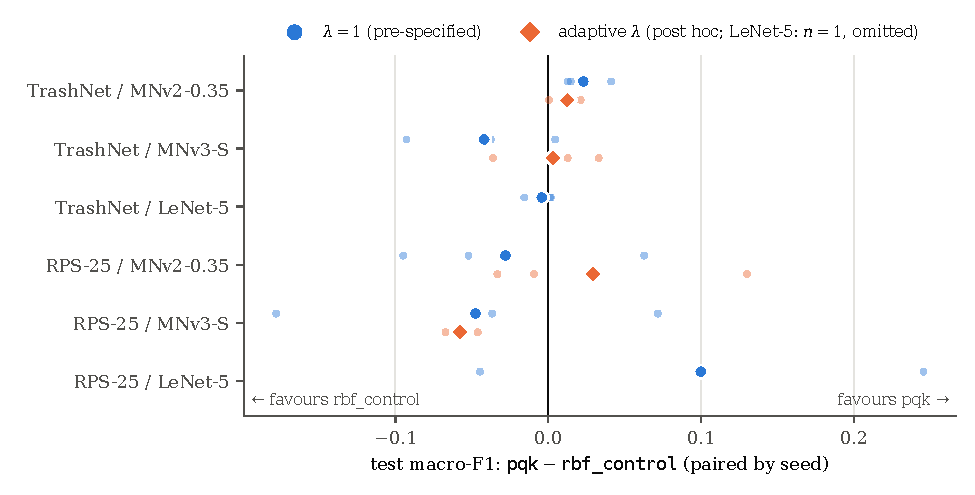
\includegraphics[width=\textwidth]{g2_paired}
  \caption{$\mathtt{pqk}-\mathtt{rbf\_control}$ per pair and seed, for the pre-specified $\lambda=1$ and for the adaptive $\lambda$ adopted after the first results. Large markers are three-seed means.}
  \label{fig:g2}
\end{figure*}

\paragraph{Against the RBF twin.}
At the pre-specified $\lambda=1$, \Pqk is ahead of its twin on the mean in only \GtwoFixedWins{} of \NPairs{} pairs (Table~\ref{tab:g2}, Figure~\ref{fig:g2}). These are TrashNet/MobileNetV2-0.35 ($+0.023\pm0.016$, three of three seeds) and RPS-25/LeNet-5 ($+0.100\pm0.145$, two of three). It is behind on the other four ($-0.042$, $-0.004$, $-0.028$, $-0.048$).
The two pairs it wins are the two that were evaluated first. Four further pairs did not reproduce them.
With the adaptive $\lambda$, which gives \Pqk the same calibration as the twin, \Pqk is ahead on \GtwoAdaptWins{} of \GtwoAdaptPairs{} pairs ($+0.013\pm0.011$, $+0.003\pm0.036$, $+0.029\pm0.088$) and behind on RPS-25/MobileNetV3-Small ($-0.058\pm0.011$). It wins on $3$, $2$, $1$ and $0$ seeds of three respectively, so the second and third winning means rest on one or two seeds.
The smallest $p$-value for $\lambda=1$ is \MinPRbfFixed{}. For the adaptive variant it is \MinPRbfAdapt{}, on RPS-25/MobileNetV3-Small, where the difference favours \MinPRbfAdaptFavours.
The quantum kernel shows no consistent advantage over its classical counterpart.

\begin{table*}[t]
  \centering
  \caption{Paired difference $\mathtt{pqk}-\mathtt{rkd}$ in test macro-F1. \Rkd was not part of the final grid for RPS-25/LeNet-5.}
  \label{tab:pqk-rkd}
  \adjustbox{max width=0.85\textwidth}{\begin{tabular}{@{}llcc@{}}
\toprule
Dataset & Student & \texttt{rkd} & $\Delta$ \texttt{pqk} $-$ \texttt{rkd} \\
\midrule
TrashNet & MobileNetV2-0.35 & $0.672\pm0.004$ & $+0.012\pm0.016$ (2/3) \\
TrashNet & MobileNetV3-S & $0.716\pm0.003$ & $+0.003\pm0.008$ (2/3) \\
TrashNet & LeNet-5 & $0.578\pm0.016$ & $-0.043\pm0.018$ (0/3) \\
RPS-25 & MobileNetV2-0.35 & $0.737\pm0.051$ & $-0.024\pm0.023$ (1/3) \\
RPS-25 & MobileNetV3-S & $0.849\pm0.048$ & $-0.009\pm0.111$ (1/3) \\
RPS-25 & LeNet-5 & -- & -- \\
\bottomrule
\end{tabular}
}
\end{table*}

\paragraph{Against relational KD.}
QRKD is a quantum extension of RKD, so \Rkd is the classical ancestor of \Pqk (Table~\ref{tab:pqk-rkd}).
\Pqk is ahead of \Rkd on the two TrashNet MobileNet pairs ($+0.012\pm0.016$ and $+0.003\pm0.008$). It is behind on TrashNet/LeNet-5 ($-0.043\pm0.018$, behind on every seed, $p=0.052$), RPS-25/MobileNetV2-0.35 ($-0.024\pm0.023$) and RPS-25/MobileNetV3-Small ($-0.009\pm0.111$).
That is \RkdAhead{} of \RkdPairs{} pairs, by at most \RkdMaxLead{} macro-F1.
The setting differs from that of QRKD, so this is not a failed replication. We do not observe consistent gains over classical relational distillation.

\subsection{Seed-to-seed variance}
\label{sec:results-variance}

\begin{table*}[t]
  \centering
  \caption{Standard deviation of test macro-F1 across the three seeds. Bold: lowest of the five methods, with \Pqk at its validation-selected $\lambda$ (last column); the two fixed and adaptive columns show both calibrations. The last row is the root mean square over pairs (adaptive: four pairs, \Rkd: five). $^{\S}$,$^{\P}$See Table~\ref{tab:main}.}
  \label{tab:var}
  \adjustbox{max width=\textwidth}{\begin{tabular}{@{}llccccccc@{}}
\toprule
Dataset & Student & \texttt{scratch} & \texttt{kd} & \texttt{rkd} & \texttt{rbf\_control} & \texttt{pqk} $\lambda{=}1$ & \texttt{pqk} adaptive & \texttt{pqk} selected \\
\midrule
TrashNet & MobileNetV2-0.35 & $0.014$ & $0.013$ & $\mathbf{0.004}$ & $0.010$ & $0.006$ & $0.013$ & $0.013$ \\
TrashNet & MobileNetV3-S & $0.016$ & $0.020$ & $\mathbf{0.003}$ & $0.037$ & $0.023$ & $0.009$ & $0.009$ \\
TrashNet & LeNet-5 & $0.021$ & $0.074$ & $0.016$ & $0.008$ & $0.003$ & -- & $\mathbf{0.003}$ \\
RPS-25 & MobileNetV2-0.35 & $\mathbf{0.023}$ & $0.088$ & $0.051$ & $0.062$ & $0.031$ & $0.030$ & $0.030$ \\
RPS-25 & MobileNetV3-S & $0.053$ & $0.089$ & $\mathbf{0.048}$ & $0.063$ & $0.065$ & $0.074$ & $0.065$ \\
RPS-25 & LeNet-5 & $0.108$$^{\S}$ & $\mathbf{0.012}$$^{\P}$ & -- & $0.202$ & $0.070$ & -- & $0.070$ \\
\midrule
Pooled std (root-mean-square over pairs) & & $0.052$ & $0.060$ & $0.032$ & $0.092$ & $0.042$ & $0.041$ & $0.041$ \\
\bottomrule
\end{tabular}
}
\end{table*}

\begin{figure*}[t]
  \centering
  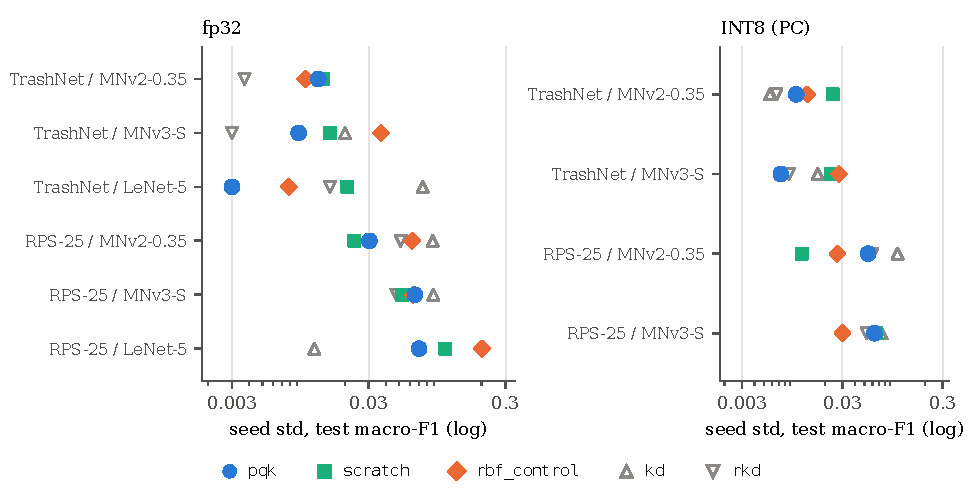
\includegraphics[width=\textwidth]{variance}
  \caption{Seed standard deviation of test macro-F1 per method and pair on a log scale, at fp32 (left) and after INT8 conversion on PC (right). \Pqk is at its validation-selected $\lambda$ at fp32 and at the exported variant at INT8.}
  \label{fig:variance}
\end{figure*}

The clearest pattern in favour of \Pqk is in the spread across seeds (Table~\ref{tab:var}, Figure~\ref{fig:variance}), and it is weaker than it first looks.
On macro-F1, with the validation-selected $\lambda$, its standard deviation is lower than that of \Rbf on \VarBelowRbf{} of \NPairs{} pairs, lower than that of \Scratch on \VarBelowScratch{}, and lower than both on three. On top-1 accuracy the counts are \VarTopBelowRbf{} and \VarTopBelowScratch{}.
Pooled over pairs (root mean square), it is \PooledPqk{} against \PooledRbf{} for \Rbf and \PooledScratch{} for \Scratch. The \Scratch figure includes the one recipe-mismatched run on RPS-25/LeNet-5\extra{ (Appendix~\ref{app:recipe})}. Without that seed the pooled \Scratch value is \PooledScratchEx{}, below that of \Pqk.
The advantage over \Rbf is the more consistent one. Against \Scratch it is fragile.
Four things limit what the pattern supports.
\emph{First}, a standard deviation from three seeds is itself very uncertain, and a sign test on four of six pairs gives $p=\SignP$.
\emph{Second}, the pattern depends on the calibration: with $\lambda=1$, \Pqk is below \Scratch on three pairs and below \Rbf on five.
\emph{Third}, it depends on the metric and on the mismatched run. Without that seed, the count against \Scratch is \VarBelowScratchEx{} of \NPairs{} on macro-F1 and \VarTopBelowScratchEx{} on top-1.
\emph{Fourth}, \Pqk is not the most stable method. On the five pairs where \Rkd exists, the pooled standard deviations are \PooledScratchFive{} for \Scratch, \PooledRkdFive{} for \Rkd and \PooledPqkFive{} for \Pqk, and \Rkd is below \Pqk on three of the five.
After INT8 conversion the pattern weakens further. Pooled over the four exported pairs on PC numerics, \Pqk has a standard deviation of \IntPooledPqk{} against \IntPooledScratch{} for \Scratch and \IntPooledRbf{} for \Rbf, because RPS-25/MobileNetV2-0.35 is noisier for \Pqk.
On TrashNet, \Pqk remains below both on both students under all three sets of kernels\extra{ (Appendix~\ref{app:int8})}.

\subsection{Entanglement and the teacher projection}
\label{sec:results-controls}

\begin{table*}[t]
  \centering
  \caption{\Pqk (adaptive $\lambda$) against the same circuit with its CNOT gates removed. Validation (decisive) and test (descriptive) macro-F1, paired by seed; $\Delta$ is $\mathtt{pqk}-\mathtt{noent\_control}$. Validation has $379$ images on TrashNet and $33$ on RPS-25.}
  \label{tab:noent}
  \adjustbox{max width=\textwidth}{\begin{tabular}{@{}llcccc@{}}
\toprule
Dataset & Student & \texttt{pqk} & no-CNOT & $\Delta$ val & $\Delta$ test \\
\midrule
TrashNet & MobileNetV2-0.35 & $0.705\pm0.006$ & $0.655\pm0.060$ & $+0.049\pm0.065$ (3/3) & $+0.059\pm0.079$ (3/3) \\
TrashNet & MobileNetV3-S & $0.737\pm0.003$ & $0.729\pm0.006$ & $+0.007\pm0.008$ (3/3) & $-0.002\pm0.028$ (1/3) \\
RPS-25 & MobileNetV2-0.35 & $0.797\pm0.083$ & $0.839\pm0.038$ & $-0.041\pm0.044$ (0/3) & $-0.060\pm0.035$ (0/3) \\
RPS-25 & MobileNetV3-S & $0.874\pm0.057$ & $0.896\pm0.037$ & $-0.022\pm0.078$ (1/3) & $-0.025\pm0.105$ (1/3) \\
\bottomrule
\end{tabular}
}
\end{table*}

\paragraph{Removing the entanglement.}
On TrashNet, whose validation split ($379$ images) is far larger than that of RPS-25, \Pqk is ahead of its entanglement-free twin on every seed of both students (validation $+0.049\pm0.065$ and $+0.007\pm0.008$, Table~\ref{tab:noent}). This is the one consistent sign that the CNOT gates contribute something beyond the sixteen trigonometric coordinates.
On RPS-25 the sign reverses ($-0.041$ and $-0.022$), on a $33$-image validation set.
Test scores point the same way except on TrashNet/MobileNetV3-Small, where the difference vanishes ($-0.002$, one seed of three).
The claim is limited.
The entanglement-free readout $(\sin4\theta,\cos4\theta)$ is highly oscillatory over $\theta\in(0,\pi)$ and may simply be a poor classical map. This result therefore does not show that \Pqk beats every classical map of equal width. The control we designed for that purpose, random Fourier features on the circuit's own frequency spectrum, was not run.
Nor did the class separation of the target kernel predict the outcome. The entanglement-free target is better aligned with the labels than the PQK target on TrashNet ($0.323$ against $0.245$ centered alignment on validation), yet students trained on the PQK target rank higher.

\begin{table*}[t]
  \centering
  \caption{Fitted minus random teacher projection, paired by seed: $\Delta$ validation and test macro-F1 for \Pqk (adaptive $\lambda$) and \Rbf. Negative values favour the random projection.}
  \label{tab:fitted}
  \adjustbox{max width=\textwidth}{\begin{tabular}{@{}llcccc@{}}
\toprule
 & & \multicolumn{2}{c}{\texttt{pqk}} & \multicolumn{2}{c}{\texttt{rbf\_control}} \\
\cmidrule(lr){3-4}\cmidrule(lr){5-6}
Dataset & Student & $\Delta$ val & $\Delta$ test & $\Delta$ val & $\Delta$ test \\
\midrule
TrashNet & MobileNetV2-0.35 & $-0.049\pm0.041$ (0/3) & $-0.060\pm0.073$ (1/3) & $-0.009\pm0.016$ (1/3) & $-0.018\pm0.003$ (0/3) \\
TrashNet & MobileNetV3-S & $-0.001\pm0.020$ (1/3) & $-0.014\pm0.019$ (1/3) & $-0.037\pm0.012$ (0/3) & $-0.013\pm0.049$ (1/3) \\
RPS-25 & MobileNetV2-0.35 & $-0.087\pm0.090$ (0/3) & $-0.104\pm0.035$ (0/3) & $-0.002\pm0.050$ (1/3) & $-0.091\pm0.125$ (1/3) \\
RPS-25 & MobileNetV3-S & $+0.043\pm0.039$ (2/3) & $+0.029\pm0.133$ (2/3) & $-0.022\pm0.036$ (0/3) & $-0.053\pm0.070$ (1/3) \\
\bottomrule
\end{tabular}
}
\end{table*}

\begin{figure*}[t]
  \centering
  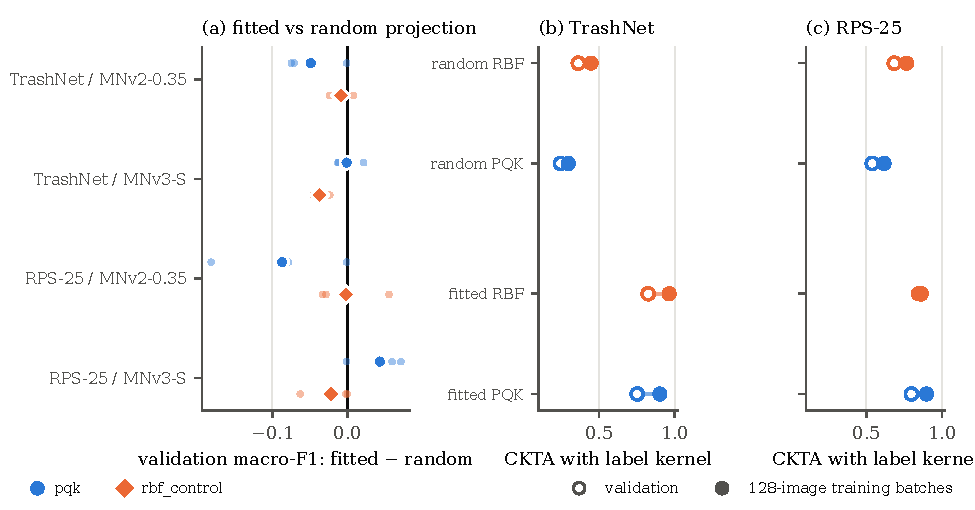
\includegraphics[width=\textwidth]{fitted_projection}
  \caption{(a)~Validation macro-F1 of a fitted (LDA+PCA) minus a random teacher projection, per seed. (b,c)~Centered kernel--target alignment (CKTA) of the target kernel the student is asked to match with the label kernel, on validation (open) and on $128$-image training batches (filled), where the loss is computed.}
  \label{fig:fitted}
\end{figure*}

\paragraph{A fitted teacher projection.}
The fixed random $2048\to8$ projection discards much of the teacher's class structure. The centered alignment of the teacher kernel with the label kernel falls from $0.720$ for the raw features to $0.363$ for the random angles on TrashNet validation.
A projection fitted on the training split (LDA+PCA) restores it ($0.825$). We selected it over PCA on validation alignment before any student was trained.
It did not help.
Fitted was better than random in \emph{one of eight} arm-pairs on validation (Table~\ref{tab:fitted}, Figure~\ref{fig:fitted}a). The exception is \Pqk on RPS-25/MobileNetV3-Small ($+0.043\pm0.039$).
The alignment measured on training batches suggests why on TrashNet.
There the fitted target is almost the label kernel on the data the loss sees: $0.963$ for the RBF target on training batches against $0.825$ on validation (random: $0.447$), and $0.902$ against $0.752$ for the PQK target (random: $0.297$ against $0.245$).
Aligning to it asks the student to cluster by class, which cross-entropy already does, and it removes the within-class geometry that relational distillation exists to transfer.
On RPS-25 the picture is mixed, and this account does not explain it. The fitted RBF target is not saturated on training batches ($0.844$ against $0.861$ on validation). The fitted PQK target is more aligned on training batches than on validation ($0.897$ against $0.797$), and that arm produced the one positive case.
The saturation account therefore covers the TrashNet results only. It is a hypothesis supported by the measurement, and we did not test it by intervention.
The measurement also shows that the selection criterion, validation alignment, was the wrong one for a relational target, because it rewards class separation.

\begin{figure*}[t]
  \centering
  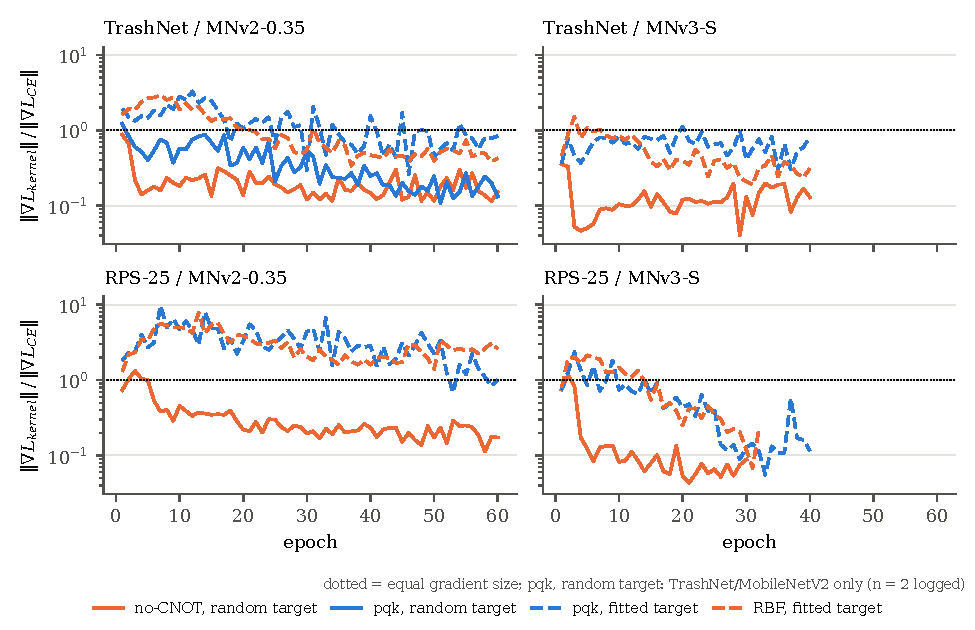
\includegraphics[width=\textwidth]{gradient_balance}
  \caption{Ratio of the gradient norm of the kernel term to that of the cross-entropy term, on the first batch of each epoch, averaged over seeds. Dashed lines use the fitted teacher projection. The solid blue line (\Pqk with a random target) was logged for TrashNet/MobileNetV2-0.35 only.}
  \label{fig:grad}
\end{figure*}

\paragraph{Does the kernel term dominate training?}
Not with the random target.
For the entanglement-free arm (12 runs), the ratio of the kernel gradient to the cross-entropy gradient falls from a mean of $0.70$ over the first three epochs to $0.14$ over the last five. For \Pqk, which was logged for only two runs (TrashNet/MobileNetV2-0.35; Figure~\ref{fig:grad}), it falls from $0.88$ to $0.20$. The label and logit terms therefore drive training after the first epochs.
With a fitted target the ratio over the last five epochs is $0.74$, $0.62$ and $0.34$ for \Pqk and $0.45$, $0.30$ and $0.28$ for \Rbf on TrashNet/MobileNetV2-0.35, TrashNet/MobileNetV3-Small and RPS-25/MobileNetV3-Small. On RPS-25/MobileNetV2-0.35 it is $3.1$ and $2.1$, and the kernel term outweighs the label signal.

\subsection{INT8 conversion}
\label{sec:results-int8}

\begin{table*}[t]
  \centering
  \caption{Change in test macro-F1 from fp32 to INT8, pooled over the exported pairs and seeds (mean, and the number of the 12 models whose score rose), for each method and set of kernels.}
  \label{tab:int8-delta}
  \adjustbox{max width=0.85\textwidth}{\begin{tabular}{@{}lccc@{}}
\toprule
Method & PC (builtin) & Pi builtin & Pi XNNPACK \\
\midrule
\texttt{scratch} & $+0.0058$ (7/12) & $+0.0038$ (7/12) & $+0.0011$ (5/12) \\
\texttt{kd} & $-0.0031$ (5/12) & $-0.0027$ (5/12) & $-0.0049$ (4/12) \\
\texttt{rkd} & $+0.0030$ (6/12) & $+0.0033$ (6/12) & $-0.0011$ (5/12) \\
\texttt{rbf\_control} & $-0.0064$ (5/12) & $-0.0045$ (5/12) & $+0.0006$ (6/12) \\
\texttt{pqk} & $+0.0080$ (9/12) & $+0.0088$ (9/12) & $+0.0025$ (5/12) \\
\bottomrule
\end{tabular}
}
\end{table*}

\begin{figure*}[t]
  \centering
  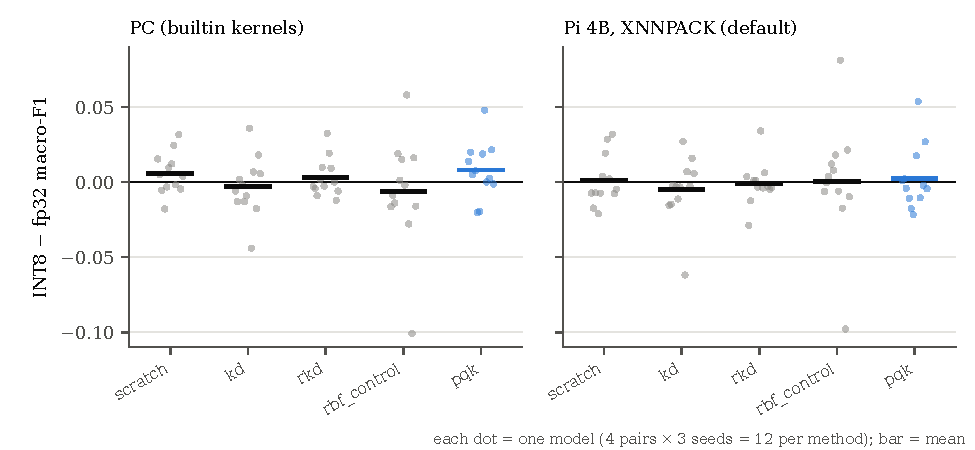
\includegraphics[width=\textwidth]{int8_delta}
  \caption{INT8 minus fp32 test macro-F1 for every exported model, by method, on PC and with the Pi's default kernels. Each dot is one model; bars are means.}
  \label{fig:int8}
\end{figure*}

All \NIntModels{} exported models pass every check. They are fully integer, quantized per channel on every convolution, contain no custom or floating-point operations, and reproduce their fp32 score exactly on reload. Their ONNX graphs match the PyTorch logits to within $1.3\times10^{-4}$\extra{ (Appendix~\ref{app:export})}.
Their size is set by the architecture alone: \MbMnvTwo{}\,MB ($604$--$608$\,KiB) for MobileNetV2-0.35 and \MbMnvThree{}\,MB ($1179$--$1181$\,KiB) for MobileNetV3-Small. Any comparison at matched size therefore holds by construction.
Conversion has no systematic cost. The macro-F1 changes by $\IntDeltaMean\pm\IntDeltaStd$ across the \NIntModels{} models, and \IntGained{} of them improve.
Conversion does change predictions. The INT8 and fp32 models disagree on about $7\%$ of test images ($91.5\%$ agreement for MobileNetV2-0.35 and $95.3\%$ for MobileNetV3-Small), in both directions.
INT8 rankings between methods are therefore fp32 rankings plus noise.
\Pqk has the most favourable change of the five methods on PC numerics ($+0.0080$, up on $9$ of $12$ models, against $-0.0031$ and $5$ of $12$ for \Kd). The difference between the two changes is not significant ($p=\QuantPPc{}$ on PC, \QuantPBuiltin{} on the Pi's builtin kernels, \QuantPXnn{} with XNNPACK), and it shrinks to $+0.0025$ with the Pi's default kernels (Table~\ref{tab:int8-delta}, Figure~\ref{fig:int8}).
The sign of other methods' changes also depends on the kernels: \Rbf moves from $-0.0064$ on PC to $+0.0006$ with XNNPACK, and \Rkd from $+0.0030$ to $-0.0011$.

\subsection{On-device behaviour}
\label{sec:results-device}

\begin{table*}[t]
  \centering
  \caption{INT8 models on the Raspberry Pi 4B with the default XNNPACK delegate, four threads, batch size 1: median (p50) and 95th-percentile (p95) invocation time over $500$ calls, mean throughput, and the speed-up from one to four threads. Latency, throughput and memory are averages over the methods and seeds of each pair (15--18 models); the thread speed-up is measured on one model per pair (\Pqk, seed~0). The spread of the p50 between methods is at most $0.11$\,ms within a pair. Sizes are in KiB.}
  \label{tab:edge}
  \adjustbox{max width=\textwidth}{\begin{tabular}{@{}llrrrrrrr@{}}
\toprule
Dataset & Student & Params & INT8 KiB & MMACs & p50 ms & p95 ms & FPS & $1\!\to\!4$ thr. \\
\midrule
TrashNet & MobileNetV2-0.35 & 403{,}814 & 608 & 18.9 & 2.53 & 2.71 & 395 & $1.84\times$ \\
TrashNet & MobileNetV3-S & 930{,}470 & 1181 & 18.2 & 3.18 & 3.35 & 314 & $1.35\times$ \\
RPS-25 & MobileNetV2-0.35 & 399{,}971 & 604 & 18.9 & 2.52 & 2.73 & 395 & $1.75\times$ \\
RPS-25 & MobileNetV3-S & 928{,}739 & 1179 & 18.2 & 3.14 & 3.30 & 318 & $1.40\times$ \\
\bottomrule
\end{tabular}
}
\end{table*}

\begin{figure*}[t]
  \centering
  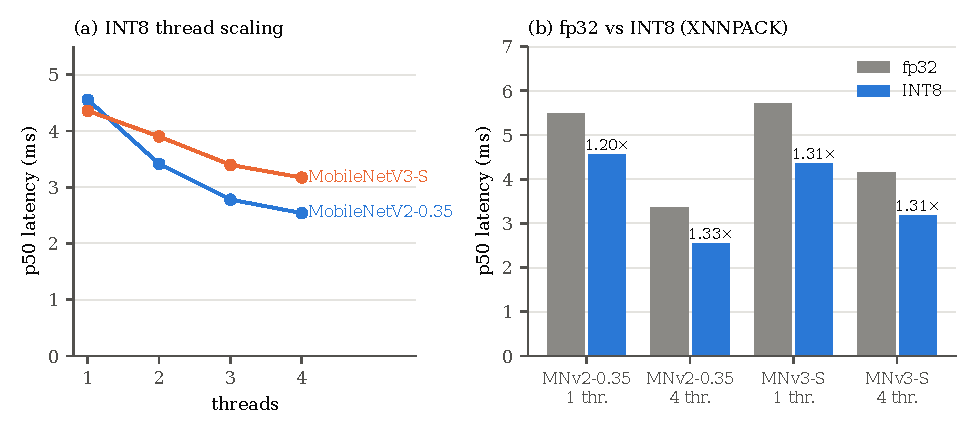
\includegraphics[width=\textwidth]{latency}
  \caption{(a)~Median INT8 latency against the number of threads. (b)~fp32 and INT8 latency with the same runtime, one and four threads, with the INT8 speed-up.}
  \label{fig:latency}
\end{figure*}

Table~\ref{tab:edge} and Figure~\ref{fig:latency} summarize the measurements ($160$ runs, none failed).
With four threads the median INT8 latency is $2.5$\,ms for MobileNetV2-0.35 and $3.2$\,ms for MobileNetV3-Small, about $395$ and $315$ inferences per second.
Latency is a property of the architecture. Within a pair, the spread between methods, which share one graph, is at most $0.11$\,ms.
The two networks do about the same work ($18.9$ and $18.2$\,M multiply--accumulates), yet MobileNetV2 is about $25\%$ faster on four threads, so operation counts do not predict speed. MobileNetV2 also scales better with threads ($1.75$--$1.84\times$ from one to four, against $1.35$--$1.40\times$), and on one thread the order reverses ($4.56$ against $4.35$\,ms on TrashNet).
Against fp32 with the same runtime (one model per pair), INT8 is $1.2$ to $1.4\times$ faster, $2.6$ to $3.1\times$ smaller, and uses less memory ($5.4$--$6.7$\,MB of interpreter memory against $8$--$12$\,MB). The speed-up is modest, and the Cortex-A72's lack of integer dot-product instructions is a likely reason.
XNNPACK is $1.1$ to $1.4\times$ faster than the builtin kernels at four threads, but it changes the model's predictions. Per model it disagrees with the PC's INT8 predictions on \XnnDisMin{}\% to \XnnDisMax{}\% of test images (\XnnDisMean{}\% on average), against at most \BuiltinDisMax{}\% (\BuiltinDisMean{}\% on average) for the builtin kernels.
It moves per-method macro-F1 by between \XnnVsPcMin{} and \XnnVsPcMax{} relative to the PC. It is also the reason the \Pqk--\Kd comparison on TrashNet/MobileNetV2-0.35 changes sign on the device ($+0.004$ on PC, $-0.004$ with XNNPACK; Table~\ref{tab:pqk-kd}).
INT8 results should therefore be reported together with the runtime that produced them.
The SoC reached at most $64.8\,^\circ$C, well below the $80\,^\circ$C throttling point. The firmware did flag an under-voltage event and a throttling event in $2$ of the $160$ runs, both at four threads, so the supply used here is marginal, and we did not attempt an energy measurement.
A live-camera pipeline\extra{ (Appendix~\ref{app:camera})} reaches about $30$ frames per second, the webcam's rate, with two inference and two OpenCV threads at $12.8$\,ms of processing per frame. Image preparation ($8.8$\,ms) costs more than inference ($4.1$\,ms). The $2.5$ and $3.2$\,ms above are invocation times only; the quantize--invoke--dequantize pipeline takes $3.4$ to $4.1$\,ms.

\subsection{Training cost}
\label{sec:results-cost}

\begin{table*}[t]
  \centering
  \caption{Compute-hours of the runs behind the reported results. Runs shared the GPU, so these are compute-hours consumed, not elapsed time, and per-epoch times are not comparable between methods. \Pqk-family hours include the CNN and the teacher forward pass, so they upper-bound the time spent simulating the circuit. Teacher fine-tuning is not included.}
  \label{tab:cost}
  \adjustbox{max width=0.9\textwidth}{\begin{tabular}{@{}lrr@{}}
\toprule
Run family & Runs kept & Compute-hours \\
\midrule
Classical (\texttt{scratch}, \texttt{kd}, \texttt{rkd}, \texttt{rbf\_control}, controls) & 98 & 49.8 \\
\texttt{pqk} family (circuit simulator in the forward pass) & 54 & 44.7 \\
\midrule
Discarded re-runs after pipeline fixes & -- & 23.0 \\
\bottomrule
\end{tabular}
}
\end{table*}

The $152$ student runs account for \CostKeptHours{} compute-hours. Of these, \CostPqkHours{} belong to the \CostPqkRuns{} runs of the \Pqk family, and a further \CostDiscardedHours{} hours went into runs discarded after pipeline fixes (Table~\ref{tab:cost}).
Because runs shared the GPU, we cannot give a clean cost ratio between methods.
The accounting does show that the circuit adds simulation to every training step of a \Pqk run, while nothing of it remains at deployment, where all methods give models of identical size and speed.

\ifextra
  \section{Discussion}
\label{sec:discussion}

\paragraph{What the evidence supports.}
Under one pipeline, with paired seeds and a classical twin, the projected quantum kernel did not separate itself from logit KD, hard-label training, relational KD or its RBF twin.
Two weak patterns favour it: a tendency to lower seed-to-seed variance (clearer against the twin than against hard-label training), and the most favourable fp32-to-INT8 change on PC numerics. Neither is significant at three seeds, and both weaken once the deployment kernels or the calibration of $\lambda$ change.
One thing does hold. Nothing quantum remains in the deployed model, because every method ends as the same plain INT8 network. A training-time quantum component therefore costs nothing at inference and, here, gains nothing there either.

\paragraph{Why the quantum map adds little.}
With the adaptive $\lambda$, the PQK Gram matrix is the median-heuristic RBF kernel on the measured features $r(\theta)$, which are sixteen fixed trigonometric polynomials of the eight angles~\citep{schuld2021effect}. The twin applies the same kernel to the angles themselves.
The two therefore differ by a fixed nonlinear map in front of identically calibrated kernels.
Such a map changes the geometry the student is asked to match, but nothing guarantees that the new geometry is more useful. We do not find that it is, which is in line with reports that tuned quantum kernels behave like classical ones~\citep{florezablan2025similarity}.
We did not measure how far apart the two Gram matrices are, and a different circuit, readout or scale could behave differently.

\paragraph{What the kernel term contributes.}
Logit KD is the only method that improves on \Scratch on every seed of the primary pairs. \Kd does so on TrashNet for both MobileNets. The classical kernel-alignment arm beats \Scratch on the mean in only \RbfBeatsScratch{} of \NPairs{} pairs, and \Pqk differs from \Scratch by at most $0.04$ in either direction.
The kernel methods carry the same logit term at a different, untuned temperature. The data therefore do not show that the logit term alone is responsible, and the asymmetry in tuning leaves the question open: the \Kd temperature was screened on some pairs, while the kernel methods share an untuned one.
With the random target, the gradient of the kernel term is a minor share of the total after the first epochs (Section~\ref{sec:results-controls}), which is consistent with a small effect on the trained network.

\paragraph{Variation between pairs.}
The sign of the difference to the twin changes from pair to pair and with the calibration of $\lambda$, and so does the best method (Section~\ref{sec:results-baselines}).
There is no clean split by dataset or architecture, and we do not identify what determines it. The differences are a few hundredths of macro-F1 against standard deviations of similar size, so much of the variation may be noise.
The two pairs examined first happened to be the two on which \Pqk looked better than its twin, and the other four did not reproduce it.
This shows how easily a few cells can mislead, which is why we report the full grid.

\paragraph{A fitted target is not a better target.}
A random projection discards much of the class structure, and making the teacher's kernel more class-separable was the natural fix. It did not help.
On TrashNet the fitted target is almost the label kernel on training batches. This suggests that it adds a second label signal while removing within-class structure. We did not test that by intervention, and the account does not explain the RPS-25 results.
Measuring alignment on training batches, and not only on validation, is a check worth making in any design that fits the target on the training data.

\paragraph{Reading the results for a deployed sorter.}
For a camera-assisted bin on a Raspberry Pi-class device, logit distillation of a MobileNet gave $0.9$ to $2.5$ points of macro-F1 over hard-label training on TrashNet, at no cost at inference. The effect of the INT8 kernels on a method's score ($\XnnVsPcMin{}$ to $\XnnVsPcMax{}$ macro-F1 between XNNPACK and the PC) is as large as several of the differences between methods.
No method here closes the gap between the best student ($0.732$) and the teacher ($0.876$).

\paragraph{Relation to QRKD.}
QRKD reports gains of a quantum-kernel relational loss over classical relational KD on MNIST, CIFAR-10 and language tasks~\citep{liu2025qrkd}.
Our setting differs in the data, the students, the loss and the controls, and we observe no consistent gain of \Pqk over \Rkd.
The two results do not conflict. Ours do suggest that gains reported without a classical kernel in the same place should be read with that control in mind.

  \section{Limitations}
\label{sec:limitations}

\begin{itemize}
  \item \textbf{Statistical power.} Each cell has three seeds. Standard deviations are poorly estimated, paired $t$-tests have little power, and none is corrected for multiple comparisons. Differences of the size we report would need many more seeds to resolve.
  \item \textbf{Exploratory status and selection.} Student recipes, the KD temperature and the RKD weights were screened on seed~0 and in part judged by test scores. The adaptive $\lambda$ was adopted after the first results. The test splits of all six pairs have therefore informed design choices, and test scores are descriptive. A confirmatory claim needs a frozen protocol, selection on validation only and fresh data.
  \item \textbf{Unmatched temperature.} The \Kd temperature was screened on TrashNet/MobileNetV2-0.35 and RPS-25/MobileNetV2-0.35 and reused for the other students of each dataset. The kernel methods share one untuned value, which may disadvantage them against \Kd. The comparison between a kernel method and its twin is matched.
  \item \textbf{Controls.} The quantum kernel is compared with one RBF twin and with the circuit without CNOT gates. A generic classical map of equal width, random Fourier features drawn from the circuit's frequency spectrum, was implemented but not run. We cannot say that \Pqk beats classical maps in general, or that it does not.
  \item \textbf{Simulation only.} The circuit is simulated without noise or shot noise at eight qubits. Nothing here concerns quantum hardware.
  \item \textbf{Scope.} We use one teacher, two datasets and three students. RPS-25 has a $33$-image validation split, so its selection and validation comparisons are weak. We did not compute calibration error, per-class recall or confusion matrices.
  \item \textbf{Recipe mismatch and omissions.} One \Scratch seed on RPS-25/LeNet-5 used a different training budget, and the \Kd cell for that pair mixes two temperatures (Appendix~\ref{app:recipe}). We did not re-run either. \Rkd is absent from the final grid for that pair because screening runs at two loss-weight scales trained poorly; their results were not retained.
  \item \textbf{Deployment.} Quantization is post-training. Only the two MobileNets are exported, and adaptive $\lambda$ has no INT8 export for TrashNet/MobileNetV2-0.35. All device results come from one Raspberry Pi~4B, whose supply triggered the firmware's under-voltage flag in $2$ of $160$ runs. Energy, the Jetson Orin Nano and the ESP32-S3 were not measured. The live-camera predictions are a demonstration on out-of-distribution frames, and the six-class and three-class models have no rejection class, so every frame receives a label.
  \item \textbf{Cost accounting.} Runs shared one GPU, so only compute-hours are reported, and the hours spent fine-tuning the teachers were not logged.
\end{itemize}

\fi
\section{Conclusion}
\label{sec:conclusion}

We asked whether a quantum kernel used only during training helps a lightweight waste classifier beyond what a classical kernel in the same place provides.
We tested this on TrashNet, with RPS-25 as a low-data confirmation, using three students and five methods under one pipeline.
A projected quantum kernel was not distinguishable from logit KD in accuracy. It was ahead on the mean in \KdAheadFp{} of \NPairs{} pairs and behind on both TrashNet MobileNets, and no paired difference was significant.
At its pre-specified scale it beat its RBF twin in \GtwoFixedWins{} of \NPairs{} pairs.
Its seed-to-seed variance tended to be lower than the twin's and, less consistently, than that of hard-label training. This tendency is not significant at three seeds, depends on the metric and on one mismatched run, and does not hold on every pair.
Removing the circuit's entanglement hurt on TrashNet validation and helped on RPS-25, and fitting the teacher projection did not help.
All \NIntModels{} exported MobileNet students are fully integer INT8 models of about \MbMnvTwo{} and \MbMnvThree{}\,MB. They run in \LatMnvTwo{} and \LatMnvThree{}\,ms per inference on a Raspberry Pi~4B, and the choice of INT8 kernels on the device changes between \XnnDisMin{}\% and \XnnDisMax{}\% of a model's predictions.
The quantum kernel leaves nothing in the deployed model, and our evidence does not show an accuracy benefit over classical alternatives.

These results are exploratory.
One question remains open: whether the quantum map beats classical maps of equal width. Answering it would need a frozen protocol, the random-feature control we did not run, at least five seeds and fresh data. On the deployment side, energy and further devices remain to be measured.


\bibliographystyle{IEEEtran}
\bibliography{references}

\ifextra
  \appendix

\section{Pitfalls We Hit and Corrected}
\label{app:pitfalls}

Three problems affected the results, and one check found none. The fixes are part of the pipeline used for every reported number.

\paragraph{BatchNorm statistics with few batches.}
A student trained from scratch on RPS-25 sees five optimization batches per epoch at batch size $128$. That is too few for BatchNorm running statistics to stabilize.
The symptom was training F1 improving normally while validation F1 stayed at one constant value, the score of a model that always predicts one class. Evaluation-mode normalization was using degenerate running statistics.
MobileNetV3-Small showed the same symptom on TrashNet, which has $14$ batches per epoch. The number of batches is therefore not the whole cause, and we did not isolate the rest.
Both cases are handled by training with per-batch statistics. Before every evaluation and before export, one no-gradient pass over the unaugmented training images accumulates cumulative running statistics, so predictions do not depend on the evaluator's batch boundaries.
This applies to all students on RPS-25, to MobileNetV3-Small on TrashNet (Table~\ref{tab:hparams-students}), and to every method alike.

\paragraph{Checkpoint selection on a small validation set.}
RPS-25's validation split has $33$ images, so validation F1 moves in steps of about three points and swings between epochs long after the model has converged.
In one screening run (MobileNetV2-0.35, KD, seed~0) the validation F1 of the first fourteen epochs was $0.53$, $0.45$, $0.31$, $0.50$, $0.52$, $0.63$, $0.64$, $0.52$, $0.60$, $0.73$, $0.74$, $0.79$, $0.82$, $0.73$. Over the same epochs the validation loss fell from $2.15$ to $1.17$ with only small reversals.
Selecting the maximum F1 picks a spike, so on RPS-25 we select by validation loss.
The kernel methods add a second effect. With the kernel weight ramped over ten epochs, the validation loss itself grows while the ramp is rising, and the least-trained epoch always looks best.
Validation is therefore scored at the final weight $\gamma_{\max}$, whatever the epoch's training weight.

\paragraph{Mutual collapse of the kernel-alignment loss.}
In our first implementation both projection heads were trainable.
Collapsing both to constant maps is then a global optimum of $\Vert\tilde K_t-\tilde K_s\Vert_F^2$. Every Gram entry becomes one, trace normalization makes the two matrices identical, and the loss is zero while the student has learned nothing.
We found the problem in the kernel statistics stored with the first \Pqk run we inspected (RPS-25, LeNet-5, seed~0; a single pass over the test split at the selected checkpoint). Its mean off-diagonal kernel value was \CollapseStudent{} for the student and \CollapseTeacher{} for the teacher. The teacher backbone is frozen and its features vary, so a value that close to one can only mean its projection had collapsed.
Two things made the problem easy to miss.
Our concentration check guarded only the vacuous end (mean off-diagonal below $0.05$) and not the saturated end. The classical twin is also immune to the symptom: the median-heuristic bandwidth rescales to the data spread in every batch and pins the off-diagonal near $0.6$ ($0.55$ to $0.63$ in the archived twin runs), however collapsed the projection is.
The twin therefore looked healthy while sharing the flaw.
The twins must share a pipeline, so every result that used the kernel pipeline before the fix was discarded and both methods were re-run. The pre-fix runs are archived, and none enters the tables.
The teacher-side projection is now frozen, and the check also flags saturation (above $0.95$).
Table~\ref{tab:kernel-health} shows the kernel statistics of the reported runs. Every arm sits between $\OffdiagOthersMin{}$ and $\OffdiagOthersMax{}$ except \Pqk with $\lambda=1$. Its mean off-diagonal value ranges from $\OffdiagFixedMin{}$ to $\OffdiagFixedMax{}$ across pairs, because a fixed $\lambda$ does not adapt to the spread of the measured features.

\begin{table*}[t]
  \centering
  \caption{Mean off-diagonal kernel value $K_{ij}$ of the student and the teacher Gram matrices, from a single pass over the test split at the selected checkpoint (averaged over its batches, at $\gamma_{\max}$), summarized over the runs of each method.}
  \label{tab:kernel-health}
  \adjustbox{max width=\textwidth}{\begin{tabular}{@{}lrcc@{}}
\toprule
Method & Runs & Student, mean [min, max] & Teacher, mean [min, max] \\
\midrule
\texttt{rbf\_control} & 20 & $0.604$ [0.557, 0.628] & $0.599$ [0.591, 0.605] \\
\texttt{noent\_control} & 12 & $0.618$ [0.610, 0.636] & $0.614$ [0.610, 0.617] \\
\texttt{pqk} & 20 & $0.500$ [0.377, 0.712] & $0.510$ [0.381, 0.680] \\
\texttt{pqk\_adaptive} & 14 & $0.609$ [0.540, 0.623] & $0.594$ [0.577, 0.607] \\
\texttt{rbf\_fit} & 12 & $0.616$ [0.581, 0.640] & $0.616$ [0.571, 0.661] \\
\texttt{pqk\_fit} & 12 & $0.615$ [0.589, 0.637] & $0.621$ [0.593, 0.649] \\
\bottomrule
\end{tabular}
}
\end{table*}

\paragraph{A check that found no problem: gradient size of the kernel term.}
We checked whether the kernel term could crowd out the label signal after the ramp, by logging per-term gradient norms (Figure~\ref{fig:grad}). With a random target it does not. With a fitted target it did on RPS-25/MobileNetV2-0.35 (Section~\ref{sec:results-controls}).

\section{Selecting the Scale of the Quantum Kernel}
\label{app:screens}

The pre-specified $\lambda=1$ gave the \Pqk results of the first full grid.
We added the adaptive $\lambda$ afterwards to remove an asymmetry. The twin has always recalibrated its bandwidth to each batch, whereas a fixed $\lambda$ left \Pqk with a kernel sharpness that drifted across pairs (Table~\ref{tab:kernel-health}).
For each pair, we report the variant with the higher three-seed \emph{validation} macro-F1 (Table~\ref{tab:val-select}).
On RPS-25/MobileNetV3-Small the adaptive variant had earlier been chosen from a seed-0 test screen. By the three-seed validation rule, $\lambda=1$ is preferred ($0.907$ against $0.874$), and it is used.

\begin{table*}[t]
  \centering
  \caption{Validation macro-F1 of the two $\lambda$ calibrations of \Pqk (mean $\pm$ std over three seeds) and the one selected. Adaptive $\lambda$ has one seed on the LeNet-5 pairs and is not eligible there.}
  \label{tab:val-select}
  \adjustbox{max width=\textwidth}{\begin{tabular}{@{}llccc@{}}
\toprule
Dataset & Student & $\lambda{=}1$ (val.) & adaptive (val.) & selected \\
\midrule
TrashNet & MobileNetV2-0.35 & $0.692\pm0.014$ & $0.705\pm0.006$ & adaptive \\
TrashNet & MobileNetV3-S & $0.725\pm0.012$ & $0.737\pm0.003$ & adaptive \\
TrashNet & LeNet-5 & $0.567\pm0.005$ & -- ($n{=}1$) & $\lambda{=}1$ \\
RPS-25 & MobileNetV2-0.35 & $0.781\pm0.084$ & $0.797\pm0.083$ & adaptive \\
RPS-25 & MobileNetV3-S & $0.907\pm0.055$ & $0.874\pm0.057$ & $\lambda{=}1$ \\
RPS-25 & LeNet-5 & $0.858\pm0.046$ & -- ($n{=}1$) & $\lambda{=}1$ \\
\bottomrule
\end{tabular}
}
\end{table*}

We screened variants of the circuit and loss on TrashNet/MobileNetV3-Small, the pair on which \Pqk fared worst (Table~\ref{tab:screens}).
None of the changes of temperature, kernel weight or depth improved on the unmodified adaptive-$\lambda$ configuration on test macro-F1 at seed~0. On validation macro-F1 two of them were marginally above it ($\tau=3$: $0.7435$, $\gamma=0.5$: $0.7343$, against $0.7335$). These differences amount to about one to four images, and we did not pursue them.
The adaptive calibration itself raised the test macro-F1 by $0.045\pm0.033$ over $\lambda=1$, with a higher score on all three seeds. Adding two-body $\langle Z_iZ_j\rangle$ correlators to the readout changed it by $-0.009\pm0.037$ (higher on one seed of three). The gain that first appeared to come from the correlators therefore came from the calibration.
The screens also show how noisy a single seed is. On this pair the seed-0 score differs from the three-seed mean by between $-0.020$ and $+0.027$ across the methods. It is above the mean by $0.027$ for $\lambda=1$ and by $0.022$ with the correlators, and below it by $0.010$ for adaptive $\lambda$. A screen on one seed can mislead in either direction.

\begin{table*}[t]
  \centering
  \caption{Variants of \Pqk on TrashNet/MobileNetV3-Small: test and validation macro-F1 at seed~0 for every variant, and the three-seed test macro-F1 where three seeds exist. Reference methods are shown for comparison.}
  \label{tab:screens}
  \adjustbox{max width=\textwidth}{\begin{tabular}{@{}llccc@{}}
\toprule
Variant & Change & seeds & seed-0 test F1 / val F1 & 3-seed test F1 \\
\midrule
\texttt{pqk} & fixed $\lambda{=}1$ (pre-specified) & 3 & $0.6998$ / $0.7377$ & $0.673\pm0.023$ \\
\texttt{pqk\_adaptive} & adaptive $\lambda$ (median heuristic) & 3 & $0.7081$ / $0.7335$ & $0.718\pm0.009$ \\
\texttt{pqk\_t3} & adaptive, $\tau{=}3$ & 1 & $0.7065$ / $0.7435$ & -- \\
\texttt{pqk\_g05} & adaptive, $\gamma{=}0.5$ & 1 & $0.6855$ / $0.7343$ & -- \\
\texttt{pqk\_g20} & adaptive, $\gamma{=}2$ & 1 & $0.6790$ / $0.7301$ & -- \\
\texttt{pqk\_d2} & adaptive, depth 2 & 1 & $0.6881$ / $0.7328$ & -- \\
\texttt{pqk\_zz} & adaptive + $\langle Z_iZ_j\rangle$ correlators & 3 & $0.7312$ / $0.7588$ & $0.709\pm0.033$ \\
\texttt{noent\_control} & no-CNOT circuit & 3 & $0.7172$ / $0.7316$ & $0.720\pm0.025$ \\
\texttt{rbf\_control} & RBF on the 8 angles & 3 & $0.6953$ / $0.7357$ & $0.715\pm0.037$ \\
\texttt{kd} & reference & 3 & $0.7239$ / $0.7538$ & $0.732\pm0.020$ \\
\texttt{scratch} & reference & 3 & $0.7119$ / $0.7293$ & $0.724\pm0.016$ \\
\bottomrule
\end{tabular}
}
\end{table*}

\section{INT8 Export Details}
\label{app:export}

\begin{table*}[t]
  \centering
  \caption{Checks on the exported models, by pair. Conv ops counts convolutions including depthwise ones. ONNX--PyTorch parity is the largest absolute logit difference over the pair's models; ``fp32 reload exact'' counts models whose reloaded fp32 weights reproduce the recorded test score. The last column is the mean change in test macro-F1 from fp32 to INT8, with its standard deviation over models.}
  \label{tab:export}
  \adjustbox{max width=\textwidth}{\begin{tabular}{@{}llrrrrrrrr@{}}
\toprule
Dataset & Student & Models & INT8 KiB & Conv ops & Integer-only & Per-channel & ONNX $\max|\Delta$logit$|$ & fp32 reload exact & INT8$-$fp32 \\
\midrule
TrashNet & MobileNetV2-0.35 & 15 & 608 & 52 & 15/15 & 15/15 & $3.6\times10^{-5}$ & 15/15 & $-0.0013\pm0.0111$ \\
TrashNet & MobileNetV3-S & 18 & 1181 & 52 & 18/18 & 18/18 & $1.6\times10^{-5}$ & 18/18 & $+0.0004\pm0.0128$ \\
RPS-25 & MobileNetV2-0.35 & 18 & 604 & 52 & 18/18 & 18/18 & $1.3\times10^{-4}$ & 18/18 & $+0.0136\pm0.0256$ \\
RPS-25 & MobileNetV3-S & 15 & 1179 & 52 & 15/15 & 15/15 & $1.0\times10^{-5}$ & 15/15 & $-0.0039\pm0.0303$ \\
\bottomrule
\end{tabular}
}
\end{table*}

Table~\ref{tab:export} summarizes the checks.
The converted graphs use only built-in integer operators.
MobileNetV2-0.35 consists of $35$ convolutions, $17$ depthwise convolutions, $10$ additions, $5$ paddings, one mean and one fully connected layer. MobileNetV3-Small consists of $41$ convolutions, $11$ depthwise convolutions, $18$ Hardswish, $9$ \texttt{RELU\_0\_TO\_1}, $9$ multiplications, $10$ means, $6$ additions, $5$ paddings and one fully connected layer.
The ONNX graphs contain only \texttt{Conv}, \texttt{Gemm}, \texttt{Add}, \texttt{Clip}, \texttt{Mul}, \texttt{Relu}, \texttt{HardSwish}, \texttt{HardSigmoid}, \texttt{Flatten}, \texttt{GlobalAveragePool} and constants.
The static batch size of one is required. A dynamic batch axis makes the converter lower \texttt{Flatten} through a \texttt{FILL} operation that strict integer quantization rejects.
We also use the converter's TensorFlow back end, because its default writer emitted invalid per-channel metadata.
The conversion used PyTorch 2.13.0, ONNX 1.20.1 and onnx2tf 2.6.9.

\section{Seed Variance at INT8 and On-Device Accuracy}
\label{app:int8}

\begin{table*}[t]
  \centering
  \caption{Seed standard deviation of INT8 test macro-F1 for the four exported pairs under the three sets of kernels. Bold: lowest of the five methods. $^{\ddagger}$The exported \Pqk is the $\lambda=1$ variant whereas the validation rule prefers adaptive $\lambda$.}
  \label{tab:var-int8}
  \adjustbox{max width=\textwidth}{\begin{tabular}{@{}lllccccc@{}}
\toprule
INT8 numerics & Dataset & Student & \texttt{scratch} & \texttt{kd} & \texttt{rkd} & \texttt{rbf\_control} & \texttt{pqk} \\
\midrule
PC (builtin) & TrashNet & MobileNetV2-0.35 & $0.024$ & $\mathbf{0.006}$ & $0.007$ & $0.013$ & $0.010$$^{\ddagger}$ \\
 & TrashNet & MobileNetV3-S & $0.023$ & $0.017$ & $0.009$ & $0.028$ & $\mathbf{0.007}$ \\
 & RPS-25 & MobileNetV2-0.35 & $\mathbf{0.012}$ & $0.106$ & $0.060$ & $0.027$ & $0.054$ \\
 & RPS-25 & MobileNetV3-S & $0.065$ & $0.074$ & $0.052$ & $\mathbf{0.030}$ & $0.063$ \\
\midrule
Pi builtin & TrashNet & MobileNetV2-0.35 & $0.024$ & $0.006$ & $\mathbf{0.005}$ & $0.015$ & $0.010$$^{\ddagger}$ \\
 & TrashNet & MobileNetV3-S & $0.022$ & $0.014$ & $0.007$ & $0.026$ & $\mathbf{0.002}$ \\
 & RPS-25 & MobileNetV2-0.35 & $\mathbf{0.012}$ & $0.106$ & $0.058$ & $0.027$ & $0.054$ \\
 & RPS-25 & MobileNetV3-S & $0.064$ & $0.072$ & $0.052$ & $\mathbf{0.029}$ & $0.065$ \\
\midrule
Pi XNNPACK & TrashNet & MobileNetV2-0.35 & $0.013$ & $\mathbf{0.007}$ & $0.019$ & $0.015$ & $0.008$$^{\ddagger}$ \\
 & TrashNet & MobileNetV3-S & $0.022$ & $0.016$ & $0.004$ & $0.033$ & $\mathbf{0.004}$ \\
 & RPS-25 & MobileNetV2-0.35 & $\mathbf{0.011}$ & $0.105$ & $0.056$ & $0.014$ & $0.062$ \\
 & RPS-25 & MobileNetV3-S & $0.069$ & $0.080$ & $0.048$ & $\mathbf{0.029}$ & $0.064$ \\
\bottomrule
\end{tabular}
}
\end{table*}

\begin{table*}[t]
  \centering
  \caption{Test macro-F1 of the exported models, mean $\pm$ std over three seeds: fp32 (recorded), INT8 on the PC, and INT8 on the Raspberry Pi with its builtin kernels and with the default XNNPACK delegate. The last column is the fraction of test images on which the XNNPACK model and the PC model predict the same class. $^{\dagger}$Adaptive $\lambda$.}
  \label{tab:device-acc}
  \adjustbox{max width=\textwidth}{\begin{tabular}{@{}lllccccc@{}}
\toprule
Dataset & Student & Method & fp32 & PC INT8 & Pi builtin & Pi XNNPACK & XNNPACK agree. \\
\midrule
TrashNet & MobileNetV2-0.35 & \texttt{scratch} & $0.684\pm0.014$ & $0.689\pm0.024$ & $0.689\pm0.024$ & $0.673\pm0.013$ & $0.946$ \\
 &  & \texttt{kd} & $0.708\pm0.013$ & $0.703\pm0.006$ & $0.703\pm0.006$ & $0.698\pm0.007$ & $0.967$ \\
 &  & \texttt{rkd} & $0.672\pm0.004$ & $0.666\pm0.007$ & $0.665\pm0.005$ & $0.659\pm0.019$ & $0.958$ \\
 &  & \texttt{rbf\_control} & $0.671\pm0.010$ & $0.658\pm0.013$ & $0.657\pm0.015$ & $0.670\pm0.015$ & $0.958$ \\
 &  & \texttt{pqk} & $0.694\pm0.006$ & $0.707\pm0.010$ & $0.707\pm0.010$ & $0.693\pm0.008$ & $0.957$ \\
\midrule
TrashNet & MobileNetV3-S & \texttt{scratch} & $0.724\pm0.016$ & $0.720\pm0.023$ & $0.715\pm0.022$ & $0.715\pm0.022$ & $0.971$ \\
 &  & \texttt{kd} & $0.732\pm0.020$ & $0.724\pm0.017$ & $0.722\pm0.014$ & $0.727\pm0.016$ & $0.977$ \\
 &  & \texttt{rkd} & $0.716\pm0.003$ & $0.718\pm0.009$ & $0.719\pm0.007$ & $0.715\pm0.004$ & $0.978$ \\
 &  & \texttt{rbf\_control} & $0.715\pm0.037$ & $0.727\pm0.028$ & $0.732\pm0.026$ & $0.728\pm0.033$ & $0.968$ \\
 &  & \texttt{pqk}$^{\dagger}$ & $0.718\pm0.009$ & $0.708\pm0.007$ & $0.706\pm0.002$ & $0.702\pm0.004$ & $0.975$ \\
\midrule
RPS-25 & MobileNetV2-0.35 & \texttt{scratch} & $0.710\pm0.023$ & $0.722\pm0.012$ & $0.722\pm0.012$ & $0.727\pm0.011$ & $0.961$ \\
 &  & \texttt{kd} & $0.710\pm0.088$ & $0.710\pm0.106$ & $0.710\pm0.106$ & $0.701\pm0.105$ & $0.945$ \\
 &  & \texttt{rkd} & $0.737\pm0.051$ & $0.757\pm0.060$ & $0.758\pm0.058$ & $0.749\pm0.056$ & $0.946$ \\
 &  & \texttt{rbf\_control} & $0.684\pm0.062$ & $0.693\pm0.027$ & $0.693\pm0.027$ & $0.703\pm0.014$ & $0.931$ \\
 &  & \texttt{pqk}$^{\dagger}$ & $0.713\pm0.030$ & $0.735\pm0.054$ & $0.735\pm0.054$ & $0.733\pm0.062$ & $0.949$ \\
\midrule
RPS-25 & MobileNetV3-S & \texttt{scratch} & $0.816\pm0.053$ & $0.826\pm0.065$ & $0.823\pm0.064$ & $0.822\pm0.069$ & $0.987$ \\
 &  & \texttt{kd} & $0.830\pm0.089$ & $0.832\pm0.074$ & $0.836\pm0.072$ & $0.836\pm0.080$ & $0.978$ \\
 &  & \texttt{rkd} & $0.849\pm0.048$ & $0.843\pm0.052$ & $0.844\pm0.052$ & $0.845\pm0.048$ & $0.991$ \\
 &  & \texttt{rbf\_control} & $0.888\pm0.063$ & $0.854\pm0.030$ & $0.857\pm0.029$ & $0.859\pm0.029$ & $0.988$ \\
 &  & \texttt{pqk} & $0.840\pm0.065$ & $0.848\pm0.063$ & $0.853\pm0.065$ & $0.847\pm0.064$ & $0.980$ \\
\bottomrule
\end{tabular}
}
\end{table*}

Table~\ref{tab:var-int8} shows the standard deviations behind Section~\ref{sec:results-variance}.
On TrashNet, \Pqk has a standard deviation below both \Scratch and \Rbf on both students under all three sets of kernels. On RPS-25 it does not.
Table~\ref{tab:device-acc} gives the scores behind Section~\ref{sec:results-device}.
With the Pi's builtin kernels the INT8 scores are within $0.006$ of the PC's. XNNPACK changes them by up to $0.016$ in either direction.

\section{Camera Pipeline and Circuit Trainability}
\label{app:camera}

\begin{figure*}[t]
  \centering
  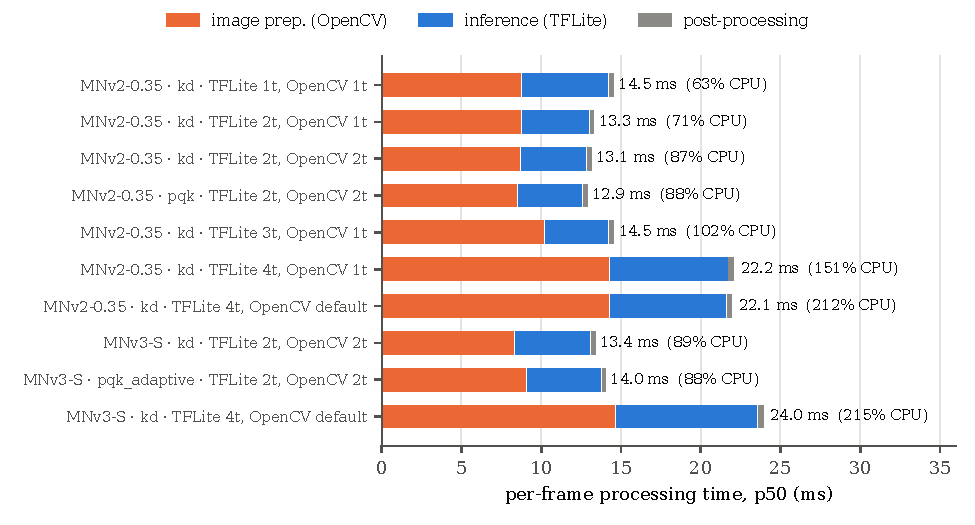
\includegraphics[width=\textwidth]{camera_pipeline}
  \caption{Median per-frame processing time of the live camera pipeline ($640{\times}480$ MJPEG) on the Raspberry Pi~4B, split into image preparation, inference and post-processing, with the process CPU use, for different thread counts.}
  \label{fig:camera}
\end{figure*}

\begin{table*}[t]
  \centering
  \caption{Live camera pipeline: median time per stage (ms), achieved frame rate and process CPU use, by number of TFLite and OpenCV threads (``default'' lets OpenCV use all cores).}
  \label{tab:camera}
  \adjustbox{max width=\textwidth}{\begin{tabular}{@{}llrrrrrrrrr@{}}
\toprule
Student & Method & TFLite thr. & CV thr. & preproc. & invoke & post & processing & FPS & CPU \% & max $^\circ$C \\
\midrule
MobileNetV2-0.35 & \texttt{kd} & 1 & 1 & 8.8 & 5.5 & 0.24 & 14.2 & 30.0 & 63 & 50.1 \\
MobileNetV2-0.35 & \texttt{kd} & 2 & 1 & 8.8 & 4.3 & 0.24 & 12.9 & 30.0 & 71 & 50.1 \\
MobileNetV2-0.35 & \texttt{kd} & 2 & 2 & 8.8 & 4.1 & 0.24 & 12.8 & 30.0 & 87 & 50.1 \\
MobileNetV2-0.35 & \texttt{kd} & 3 & 1 & 10.3 & 4.0 & 0.27 & 13.6 & 30.0 & 102 & 49.2 \\
MobileNetV2-0.35 & \texttt{kd} & 4 & 1 & 14.3 & 7.4 & 0.43 & 22.5 & 29.6 & 151 & 49.2 \\
MobileNetV2-0.35 & \texttt{kd} & 4 & 4 & 14.3 & 7.3 & 0.43 & 22.0 & 29.6 & 212 & 50.1 \\
MobileNetV2-0.35 & \texttt{pqk} & 2 & 2 & 8.6 & 4.1 & 0.24 & 12.6 & 30.0 & 88 & 49.7 \\
MobileNetV3-S & \texttt{kd} & 2 & 2 & 8.4 & 4.8 & 0.22 & 13.3 & 30.0 & 89 & 50.6 \\
MobileNetV3-S & \texttt{kd} & 4 & 4 & 14.7 & 8.9 & 0.42 & 24.1 & 28.6 & 215 & 49.2 \\
MobileNetV3-S & \texttt{pqk\_adaptive} & 2 & 2 & 9.1 & 4.7 & 0.22 & 13.5 & 30.0 & 88 & 50.1 \\
\bottomrule
\end{tabular}
}
\end{table*}

The webcam delivers about $30$ frames per second, so the pipeline is bounded by the camera whenever the processing time is below $33$\,ms.
With one to three inference threads every configuration reaches $29.99$ frames per second. The best one, two TFLite and two OpenCV threads, takes $12.8$\,ms of processing at $87\%$ CPU use.
Giving the inference all four cores raises the processing time by a factor of $1.7$ to $1.8$ ($22.0$ to $22.5$\,ms for MobileNetV2-0.35 and $24.1$\,ms for MobileNetV3-Small, against $12.8$ and $13.3$\,ms), at $150\%$ to $215\%$ CPU use. Image preparation itself slows from $8.8$ to $14.3$\,ms, and one OpenCV thread is as slow as the default.
MobileNetV3-Small then falls slightly below the camera rate ($28.6$ frames per second). We did not investigate the cause.
Image preparation ($8.8$\,ms) costs more than inference ($4.1$\,ms).
The frames come from an unconstrained scene, so the predicted classes are a demonstration, not a measurement.

\begin{figure*}[t]
  \centering
  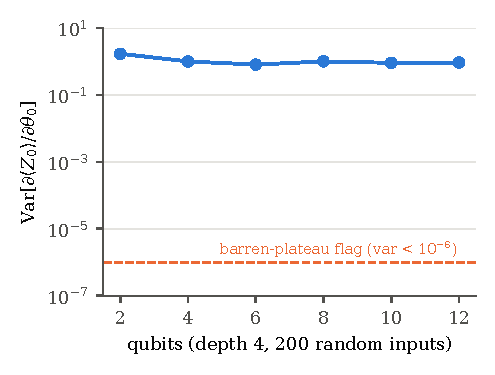
\includegraphics[width=0.55\textwidth]{barren_plateau}
  \caption{Variance of the derivative of $\langle Z_0\rangle$ with respect to the first input angle over $200$ random inputs, as a function of the number of qubits (depth $4$).}
  \label{fig:barren}
\end{figure*}

We checked that the circuit does not enter a barren-plateau regime at the width used (Figure~\ref{fig:barren}).
The gradient variance stays between $0.8$ and $1.7$ from $2$ to $12$ qubits, with no exponential decay, as expected for a shallow circuit with a local observable.
The circuit has no trainable parameters, so this concerns the gradient with respect to the input angles that reach the student.

\section{Recipe Audit}
\label{app:recipe}

Within each pair, all runs share one training recipe (epoch budget, patience, optimizer, learning rate, weight decay, batch size and BatchNorm handling), and within each cell all seeds share the loss settings.
Auditing the stored recipes found two exceptions, both on RPS-25/LeNet-5.

\paragraph{A \Scratch seed with a different budget (Table~\ref{tab:rule3}).}
Seed~0 of \Scratch on RPS-25/LeNet-5 was trained with a budget of $40$ epochs and patience $8$. The other seeds of that pair and all other methods used $60$ and $12$.
It ran all $40$ epochs, so it was limited by its budget and not stopped early. Its score is the lowest of the three.
We did not re-run it.
Excluding it makes \Scratch stronger on that pair ($0.736\pm0.044$ over the two matched seeds, against $0.676\pm0.108$ as reported), and \Pqk $-$ \Scratch goes from $-0.039$ to $-0.060$. The conclusion that \Scratch beats every distillation method there is unchanged.
The variance comparison does change. The pair's \Scratch standard deviation falls from $0.108$ to $0.044$ (two seeds), and the number of pairs on which \Pqk has a lower standard deviation than \Scratch falls from \VarBelowScratch{} to \VarBelowScratchEx{} of \NPairs{}.
Comparisons of \Pqk with \Rbf and with \Kd do not involve \Scratch and are unaffected by this run.

\paragraph{A \Kd cell with two temperatures.}
The \Kd cell for this pair mixes two settings. Seed~0 was trained at $\tau=0.5$, the temperature of the kernel methods. Seeds~1 and~2 were trained at $\tau=1$, in an earlier run at which the temperature was screened, and only seed~0 was repeated at the final value.
The three scores are $0.639$, $0.663$ and $0.649$, so the cell mean of $0.650\pm0.012$ in Table~\ref{tab:main} combines the two.
Using only the two seeds at the majority temperature, \Kd scores $0.656\pm0.010$, and \Pqk $-$ \Kd on this pair goes from $-0.013$ (as reported) to $+0.021$. On seed~0 alone it is $-0.080$.
The pair therefore flips sign depending on the seeds used. The number of pairs on which \Pqk is ahead of \Kd at fp32 is \KdAheadFp{} as reported and \KdAheadFpEx{} without seed~0.
The \Kd standard deviation for the pair, which is the lowest of any method in Table~\ref{tab:var}, mixes the two temperatures as well.
We did not re-run the two seeds, because that would require replacing stored results. The conclusion that \Pqk and \Kd are indistinguishable is unaffected, and both counts are given in the text.

\begin{table*}[t]
  \centering
  \caption{The recipe audit. $^{\S}$Run trained with a different budget and patience from the rest of its pair.}
  \label{tab:rule3}
  \adjustbox{max width=0.85\textwidth}{\begin{tabular}{@{}llrrrr@{}}
\toprule
Run & Seed & Budget & Patience & Epochs run & Macro-F1 \\
\midrule
RPS-25/LeNet-5, \texttt{scratch} & 0$^{\S}$ & 40 & 8 & 40 & $0.556$ \\
RPS-25/LeNet-5, \texttt{scratch} & 1 & 60 & 12 & 39 & $0.705$ \\
RPS-25/LeNet-5, \texttt{scratch} & 2 & 60 & 12 & 46 & $0.767$ \\
\midrule
all three seeds (as reported) & & & & & $0.676\pm0.108$ \\
matched seeds only ($n=2$) & & & & & $0.736\pm0.044$ \\
\bottomrule
\end{tabular}
}
\end{table*}

\section{Alignment of the Teacher Kernel with the Labels}
\label{app:ckta}

Table~\ref{tab:ckta} gives the centered kernel--target alignment (CKTA) between each target kernel and the label kernel $YY^{\top}$. A value of $1$ means the kernel encodes the class partition exactly.
Each target is the RBF kernel (median heuristic) of the feature map named in the row, applied to the teacher's features after the projection named in the first column.
Random projections are averaged over five draws, and fitted projections use the training split only.
The validation columns use the whole validation split. The training-batch columns use $50$ random batches of $128$ training images, which is where the loss is computed. They are computed from the teacher's features of the unaugmented training images, so they approximate the augmented batches seen in training.
The test split is never used.

\begin{table*}[t]
  \centering
  \caption{Centered kernel--target alignment of the teacher kernel with the label kernel, on validation and on $128$-image training batches.}
  \label{tab:ckta}
  \adjustbox{max width=\textwidth}{\begin{tabular}{@{}llcccc@{}}
\toprule
 & & \multicolumn{2}{c}{TrashNet} & \multicolumn{2}{c}{RPS-25} \\
\cmidrule(lr){3-4}\cmidrule(lr){5-6}
Projection & Target kernel & val. & train batches & val. & train batches \\
\midrule
-- & raw teacher 2048-d, RBF & $0.720$ & $0.818$ & $0.864$ & $0.936$ \\
\midrule
random (fixed) & angles, RBF & $0.363$ & $0.447$ & $0.684$ & $0.765$ \\
 & PQK (RY+CNOT), 16 coords & $0.245$ & $0.297$ & $0.539$ & $0.617$ \\
 & no-CNOT, 16 coords & $0.323$ & $0.408$ & $0.641$ & $0.703$ \\
\midrule
PCA (fitted) & angles, RBF & $0.666$ & $0.793$ & $0.783$ & $0.615$ \\
 & PQK (RY+CNOT), 16 coords & $0.531$ & $0.672$ & $0.754$ & $0.583$ \\
 & no-CNOT, 16 coords & $0.494$ & $0.636$ & $0.587$ & $0.480$ \\
\midrule
LDA+PCA (fitted) & angles, RBF & $0.825$ & $0.963$ & $0.861$ & $0.844$ \\
 & PQK (RY+CNOT), 16 coords & $0.752$ & $0.902$ & $0.797$ & $0.897$ \\
 & no-CNOT, 16 coords & $0.676$ & $0.855$ & $0.636$ & $0.659$ \\
\bottomrule
\end{tabular}
}
\end{table*}

\fi

\end{document}
